\section{Ideation}
Prior to our initial brainstorming session we printed a set of pictures -- each representing a specific quality, topic or idea related to our domain -- that served as a source of inspiration. We spend approximately 30 minutes finding the pictures and used sticky notes and markers to annotate interesting elements. We generally used this method as a warm-up exercise and to establish a creative atmosphere, however it also underlined the importance of light, material and structure in the home. For instance, many of the pictures depicted how light can be used to highlight unique features of a room and that high quality materials are closely connected to visual aesthetics.

\begin{figure}[h]
	\centering
	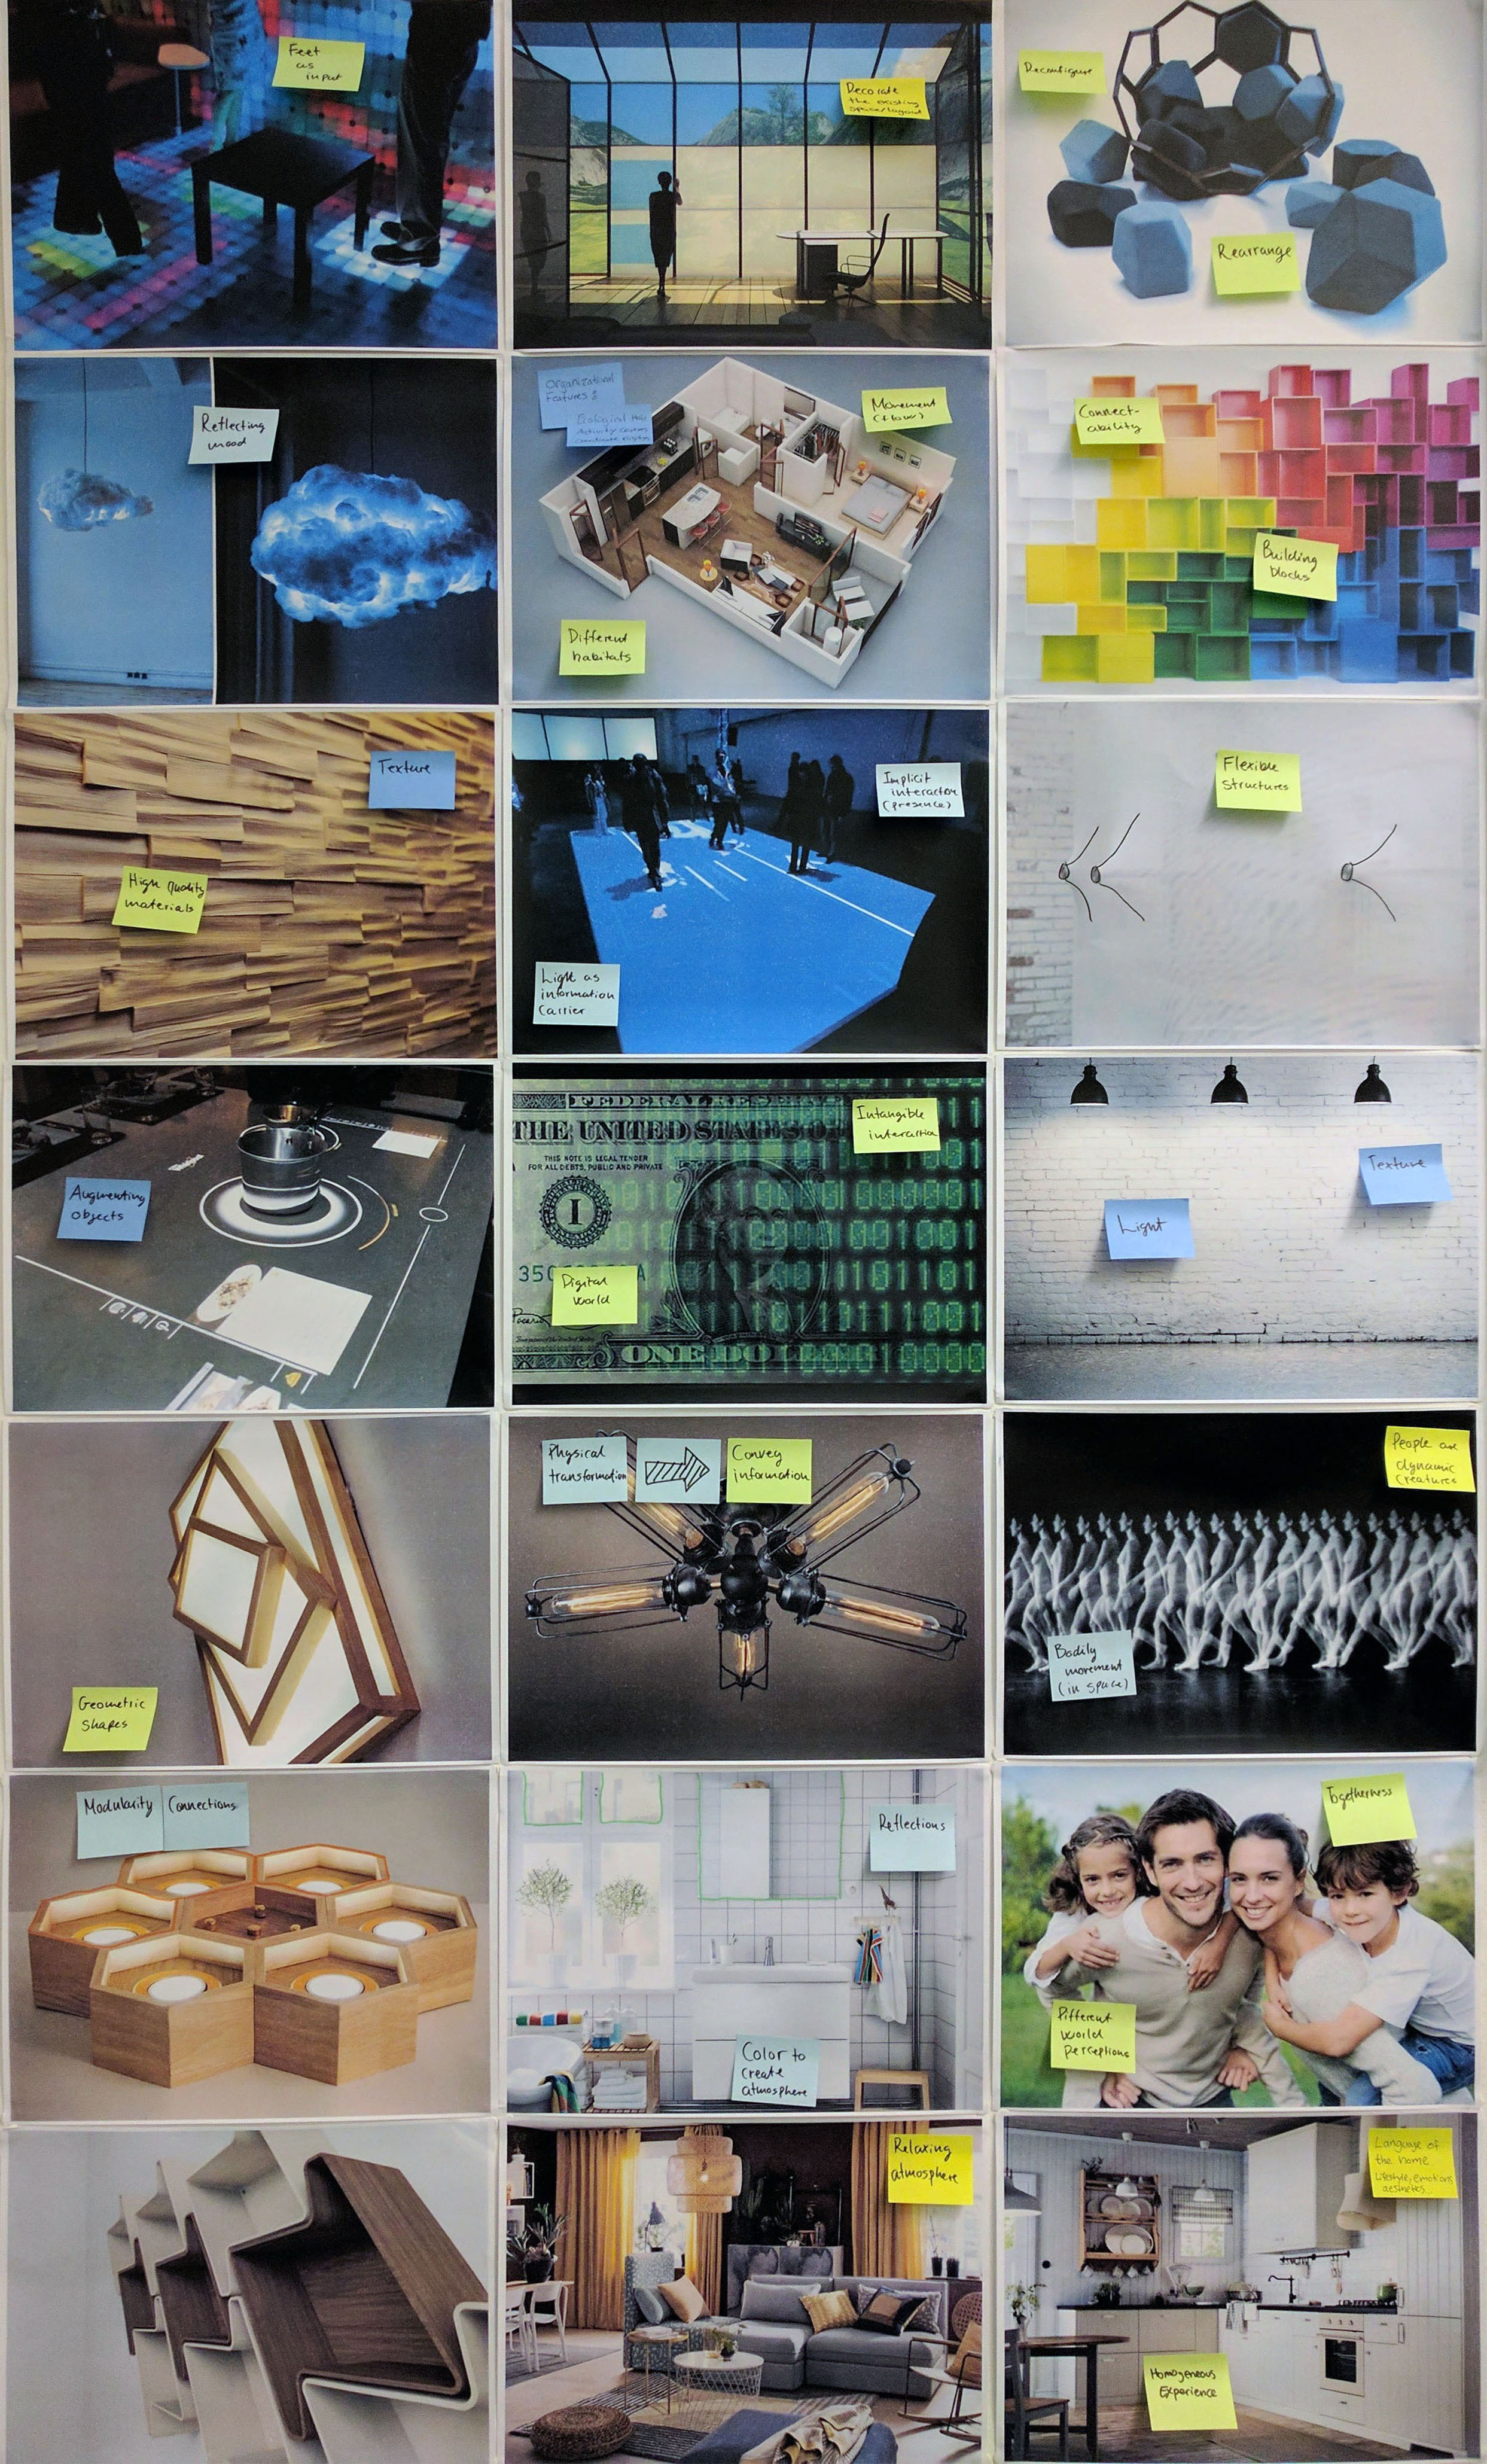
\includegraphics[width=0.5\textwidth]{picture-wall}
	\caption{Annotated pictures used to stimulate creativity}
	\label{fig:picture-wall}
\end{figure}
\subsection{Brainstorming}

In order to sharpen our focus and guide our brainstorming session we use the findings presented in section~\ref{sec:data-analysis-and-initial-findings} as categories, i.e. technology arrangements, seamless context integration, daily routines and data representation. We performed four successive brainstorming sessions lasting around 30 minutes each and used sticky notes to externalize the different ideas. Once the four brainstorming sessions ended we “dotted” the ideas -- i.e. accentuated ideas with high potential or with interesting features -- with small pieces of paper. Lastly, we discussed the different ideas, considered alternatives or combined them if we found it relevant.

\begin{figure}[h]
	\centering
	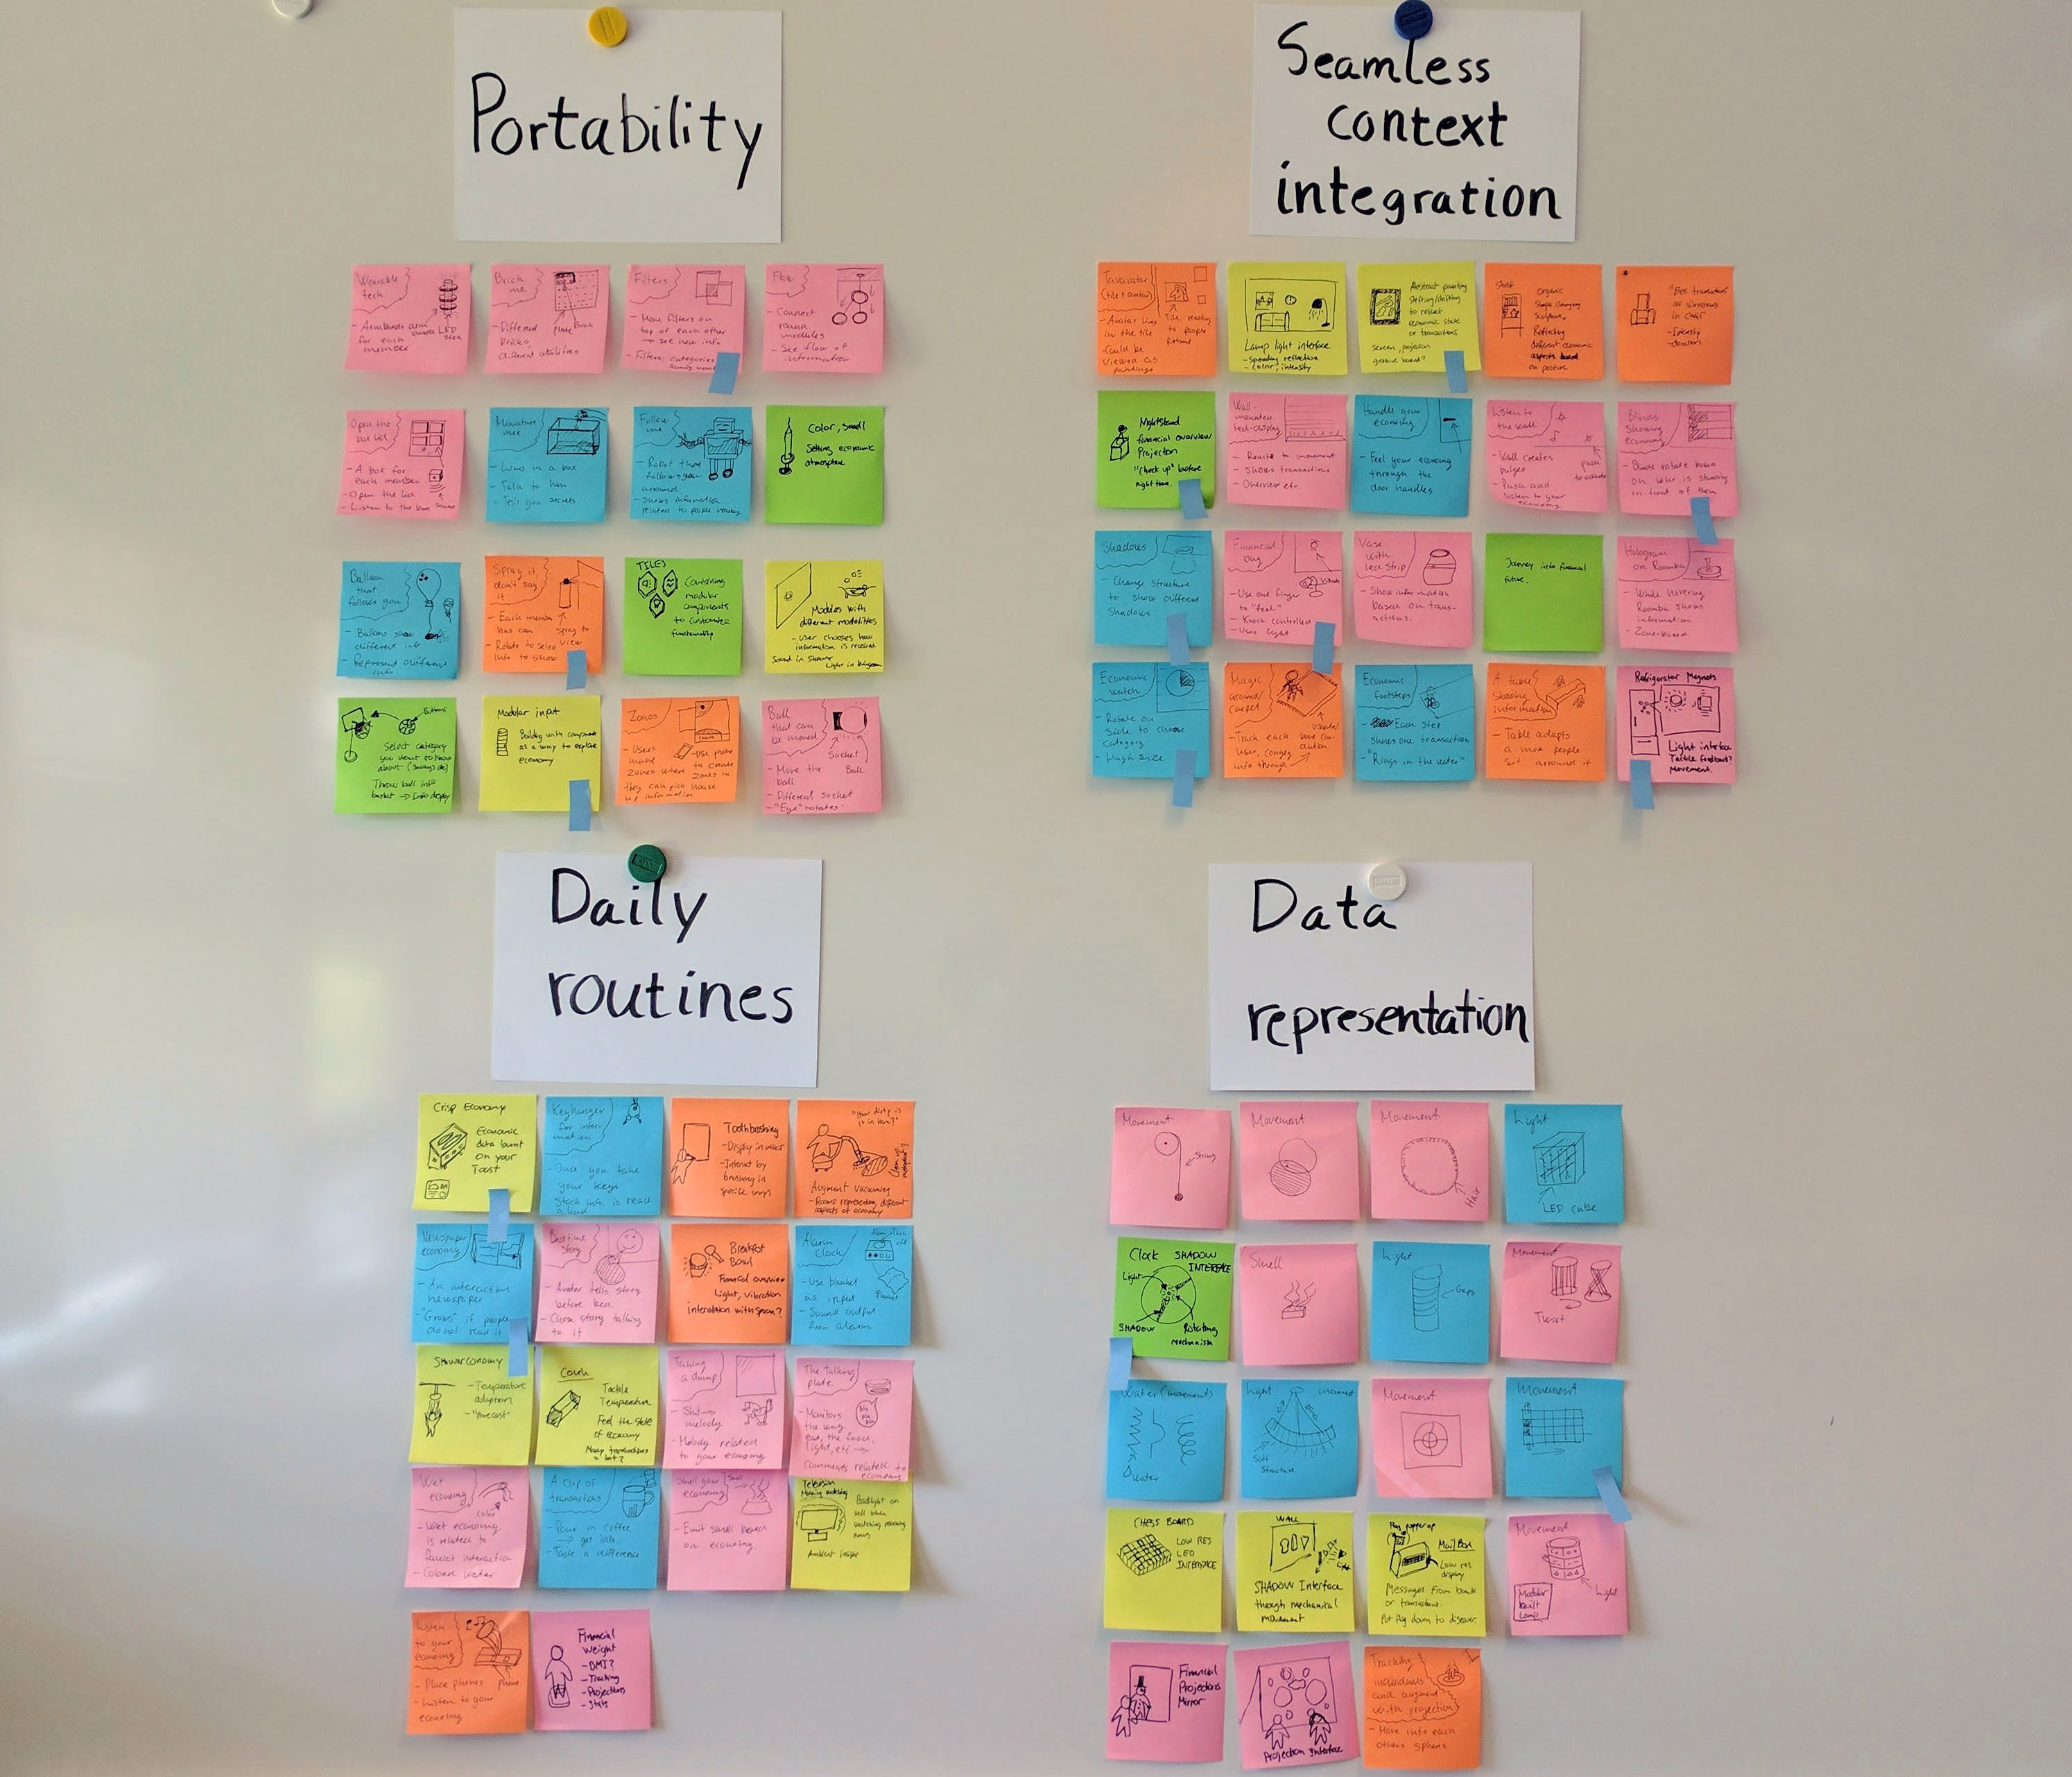
\includegraphics[width=0.75\textwidth]{brainstorming-themes}
	\caption{Outcome of the brainstorming session}
	\label{fig:brainstorming-themes}
\end{figure}

In the portability category the ideas varied greatly. Everything from a digital spray can which could be used to “paint” walls with financial information to candles emitting smell and light to create an “economic atmosphere” was purposed. However, one of the most prominent themes within this category was configurability meaning that many of the artifacts could be adapted to different circumstances and people, and therefore we decided to investigate this direction further. In the seamless context integration category two main themes surfaced, namely augmenting the infrastructure of the home (walls, floors, windows, doors, etc.) and self-contained household objects (tables, chairs, wall clocks, etc.). One of the ideas within this category utilized natural light from a window to create a type of a shadow display that would reflect significant changes in the economy. A second idea was a type of financial clock that would display various financial interactions -- we found this concept particularly interesting due to its strong connection to time. The ideas from the third category, daily routines, tried to weave financial data into ordinary routines. Especially morning routines seemed to be prevalent as many of the ideas depicted objects for a waking up or breakfast experience, e.g. a toaster burning financial information into bread or an alarm clock playing financial tunes. The fourth category, data representation, deviated slightly from the other categories as it mainly showcased different displays or mechanisms without specifying how they were connected to economy. It mainly consisted of physical moving structures that could be used to display information in varying levels of detail. Since this category did not contain any concrete concepts related to economy we decided not to pursue this direction with a specific prototype.

\subsection{Three Possible Directions}
As described in the previous section, the outcome of the brainstorming session was choosing three distinct ideas to pursue further, each with a strong focus on a specific emergent theme. The reasoning behind this was to discover which themes were most promising and significant in designing financial management technology for the home. Naturally each idea has connotations to other themes as they are intertwined to some extent but the ideas were chosen deliberately for their particularly apparent connection to the themes of daily routines, seamless context integration and portability, respectively. Two of the prototypes work explicitly with the subject of financial status because we found that users value knowledge about the status of their spendings and that it is strongly related to feeling economically aware. The three ideas will be presented briefly followed by an evaluation of the ideas with a group of former workshop participants.

\subsubsection*{Coffee Mug for a Morning Routine}
The Coffee Mug prototype (see figure figure~\ref{fig:coffee-mug}) focuses explicitly on providing a brief financial overview as part of a morning routine that many people have in common, namely drinking coffee for breakfast. The mug features a compartment in the bottom that is connected to the handle. This compartment is filled with liquid and contains a pressure system enabling it to regulate the liquid level in the handle. The liquid level represents the user’s monthly spending budget with a full handle equating no money spent and an empty handle meaning that the monthly budget has been spent. The Coffee Mug, thus enables the user to get an approximate status of the monthly budget at a glance as part of his morning routine.

\begin{figure}[h]
	\centering
	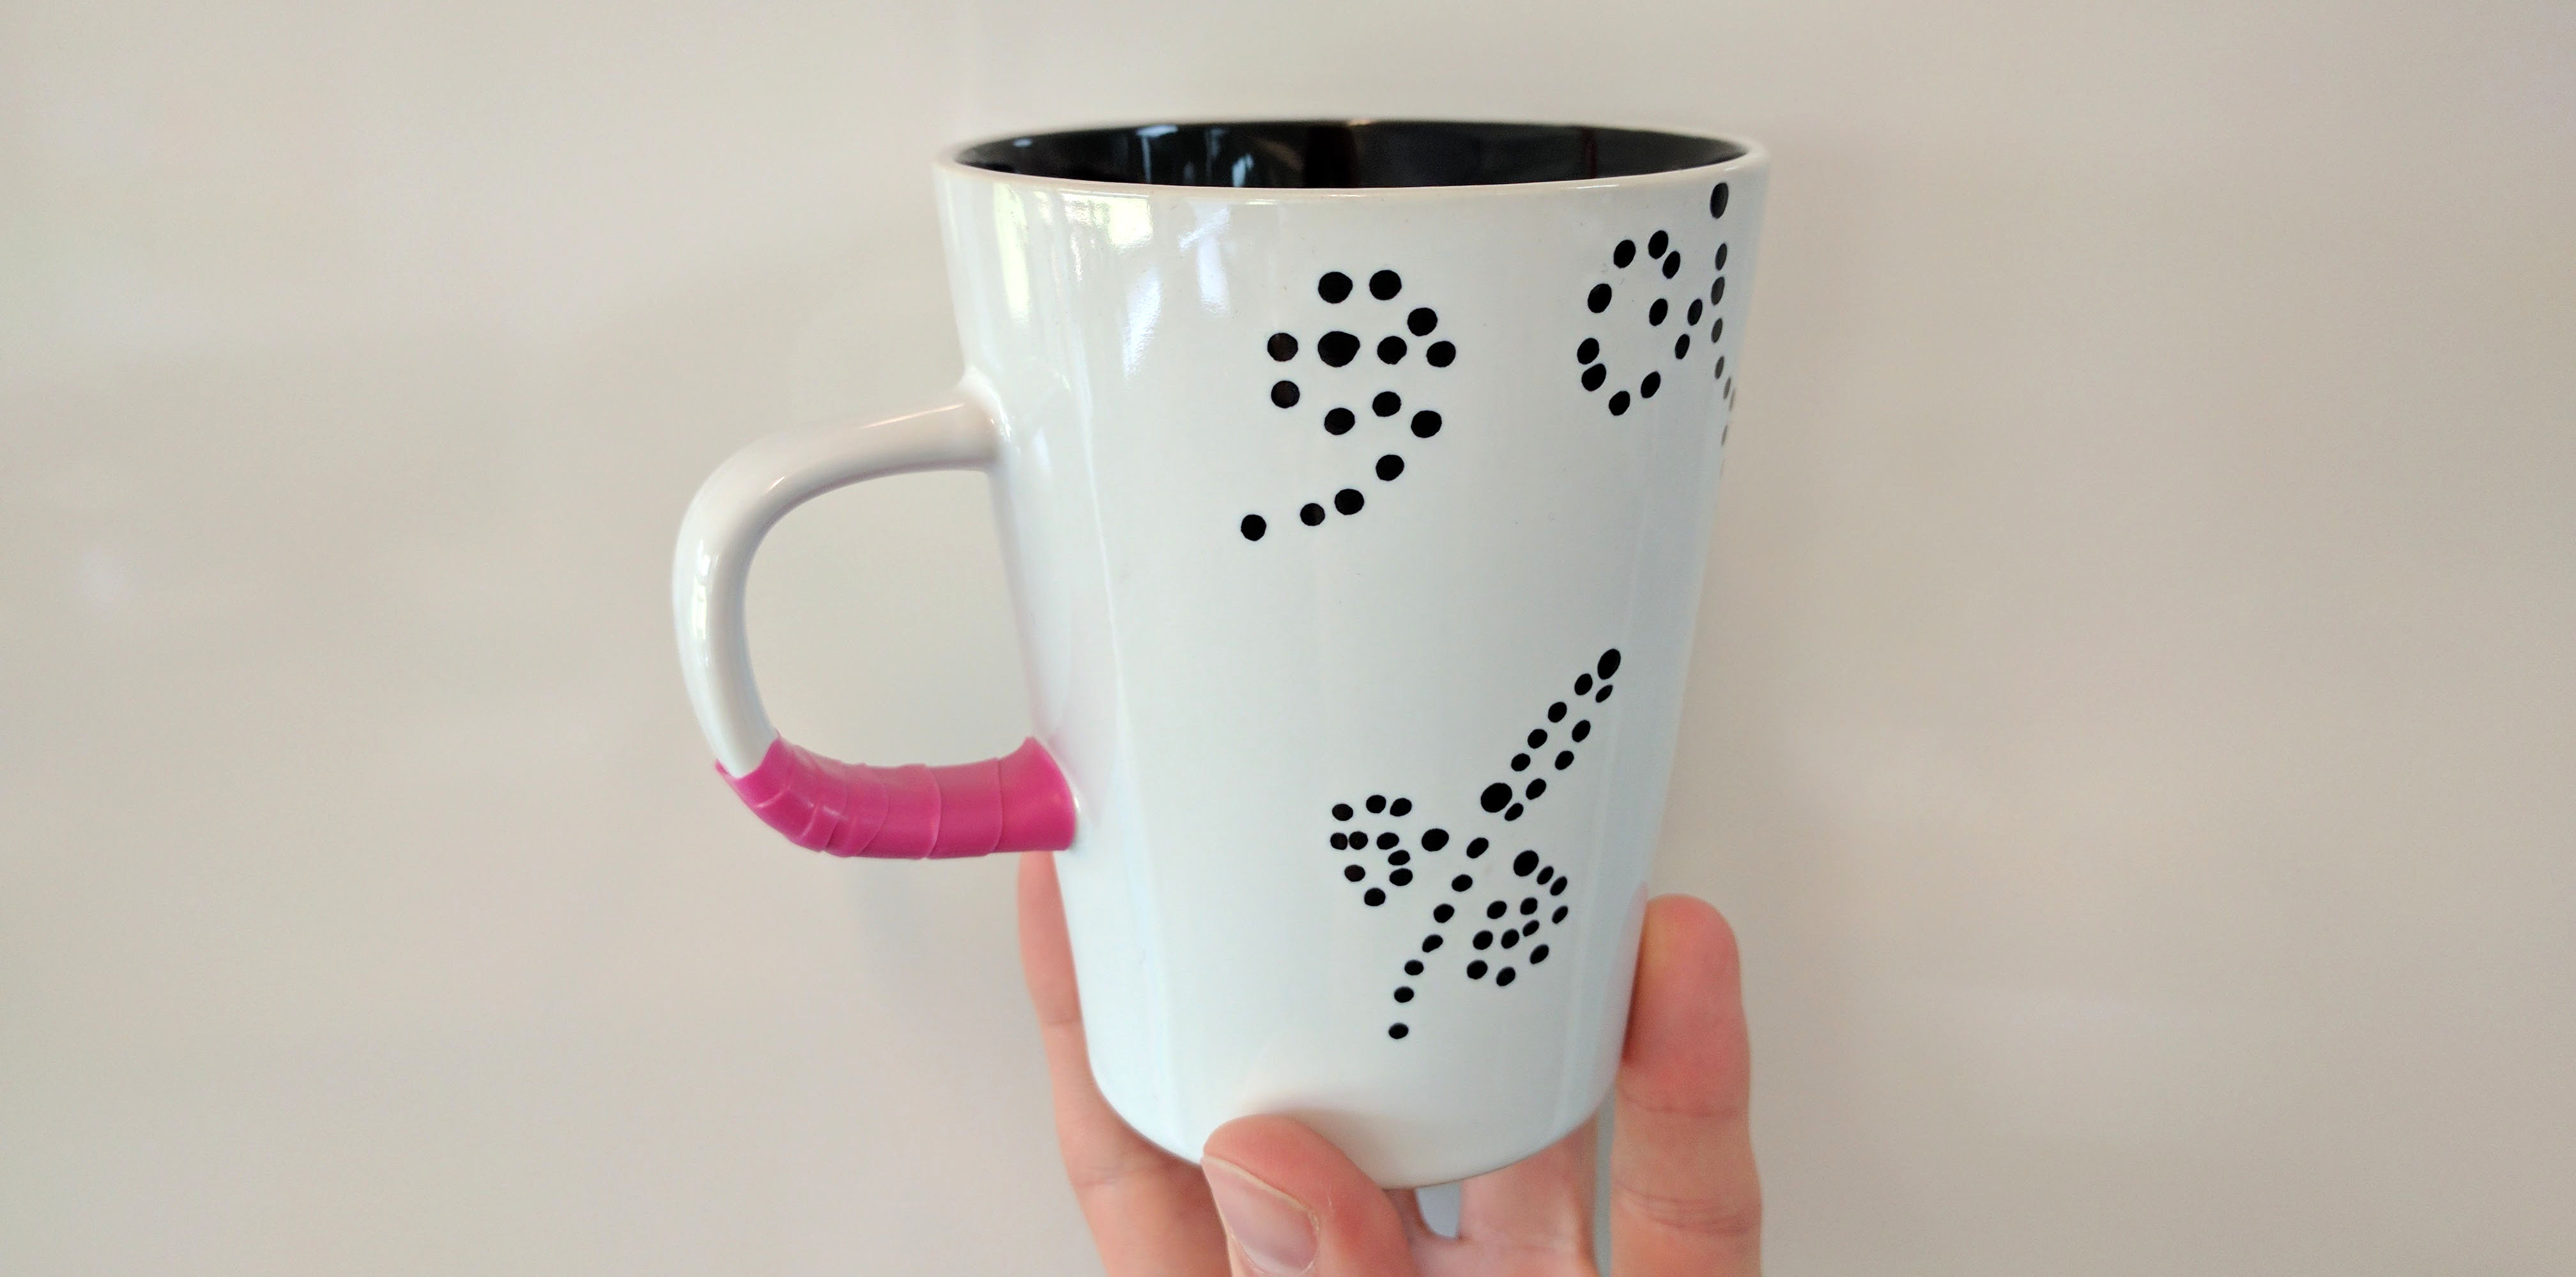
\includegraphics[width=0.75\textwidth]{coffee-mug}
	\caption{Coffee Mug prototype presenting a brief overview of monthly spending as a part of the morning routine}
	\label{fig:coffee-mug}
\end{figure}

\subsubsection*{Financial Clock}
\label{sec:financial-clock-concept}
Focusing on the theme of seamless context integration we chose to work with a clock as it is an object that is installed in the home and lives among the other household objects, thus being well integrated in the context. The Financial Clock prototype consists of a display that covers the entire dial, a center display and an interactive clock hand (see figure figure~\ref{fig:financial-clock-low-fi}). One revolution on the dial represents the user’s monthly spending budget. The dial is filled with slices, starting from twelve o’clock, that differ in size relative to the transactions they depict. The clock hand is placed on the bezel of the clock and rotates as on a regular clock but with one revolution taking a month instead of 24 hours. This makes it easy to spot whether the spendings are on track with the budget, as the transaction slices and clock hand should follow each other around the clock. The user can furthermore inspect the individual transactions by rotating the clock hand to point at the slice of interest. The transaction corresponding to that particular slice is then shown in the center display.

\begin{figure}[h]
	\centering
	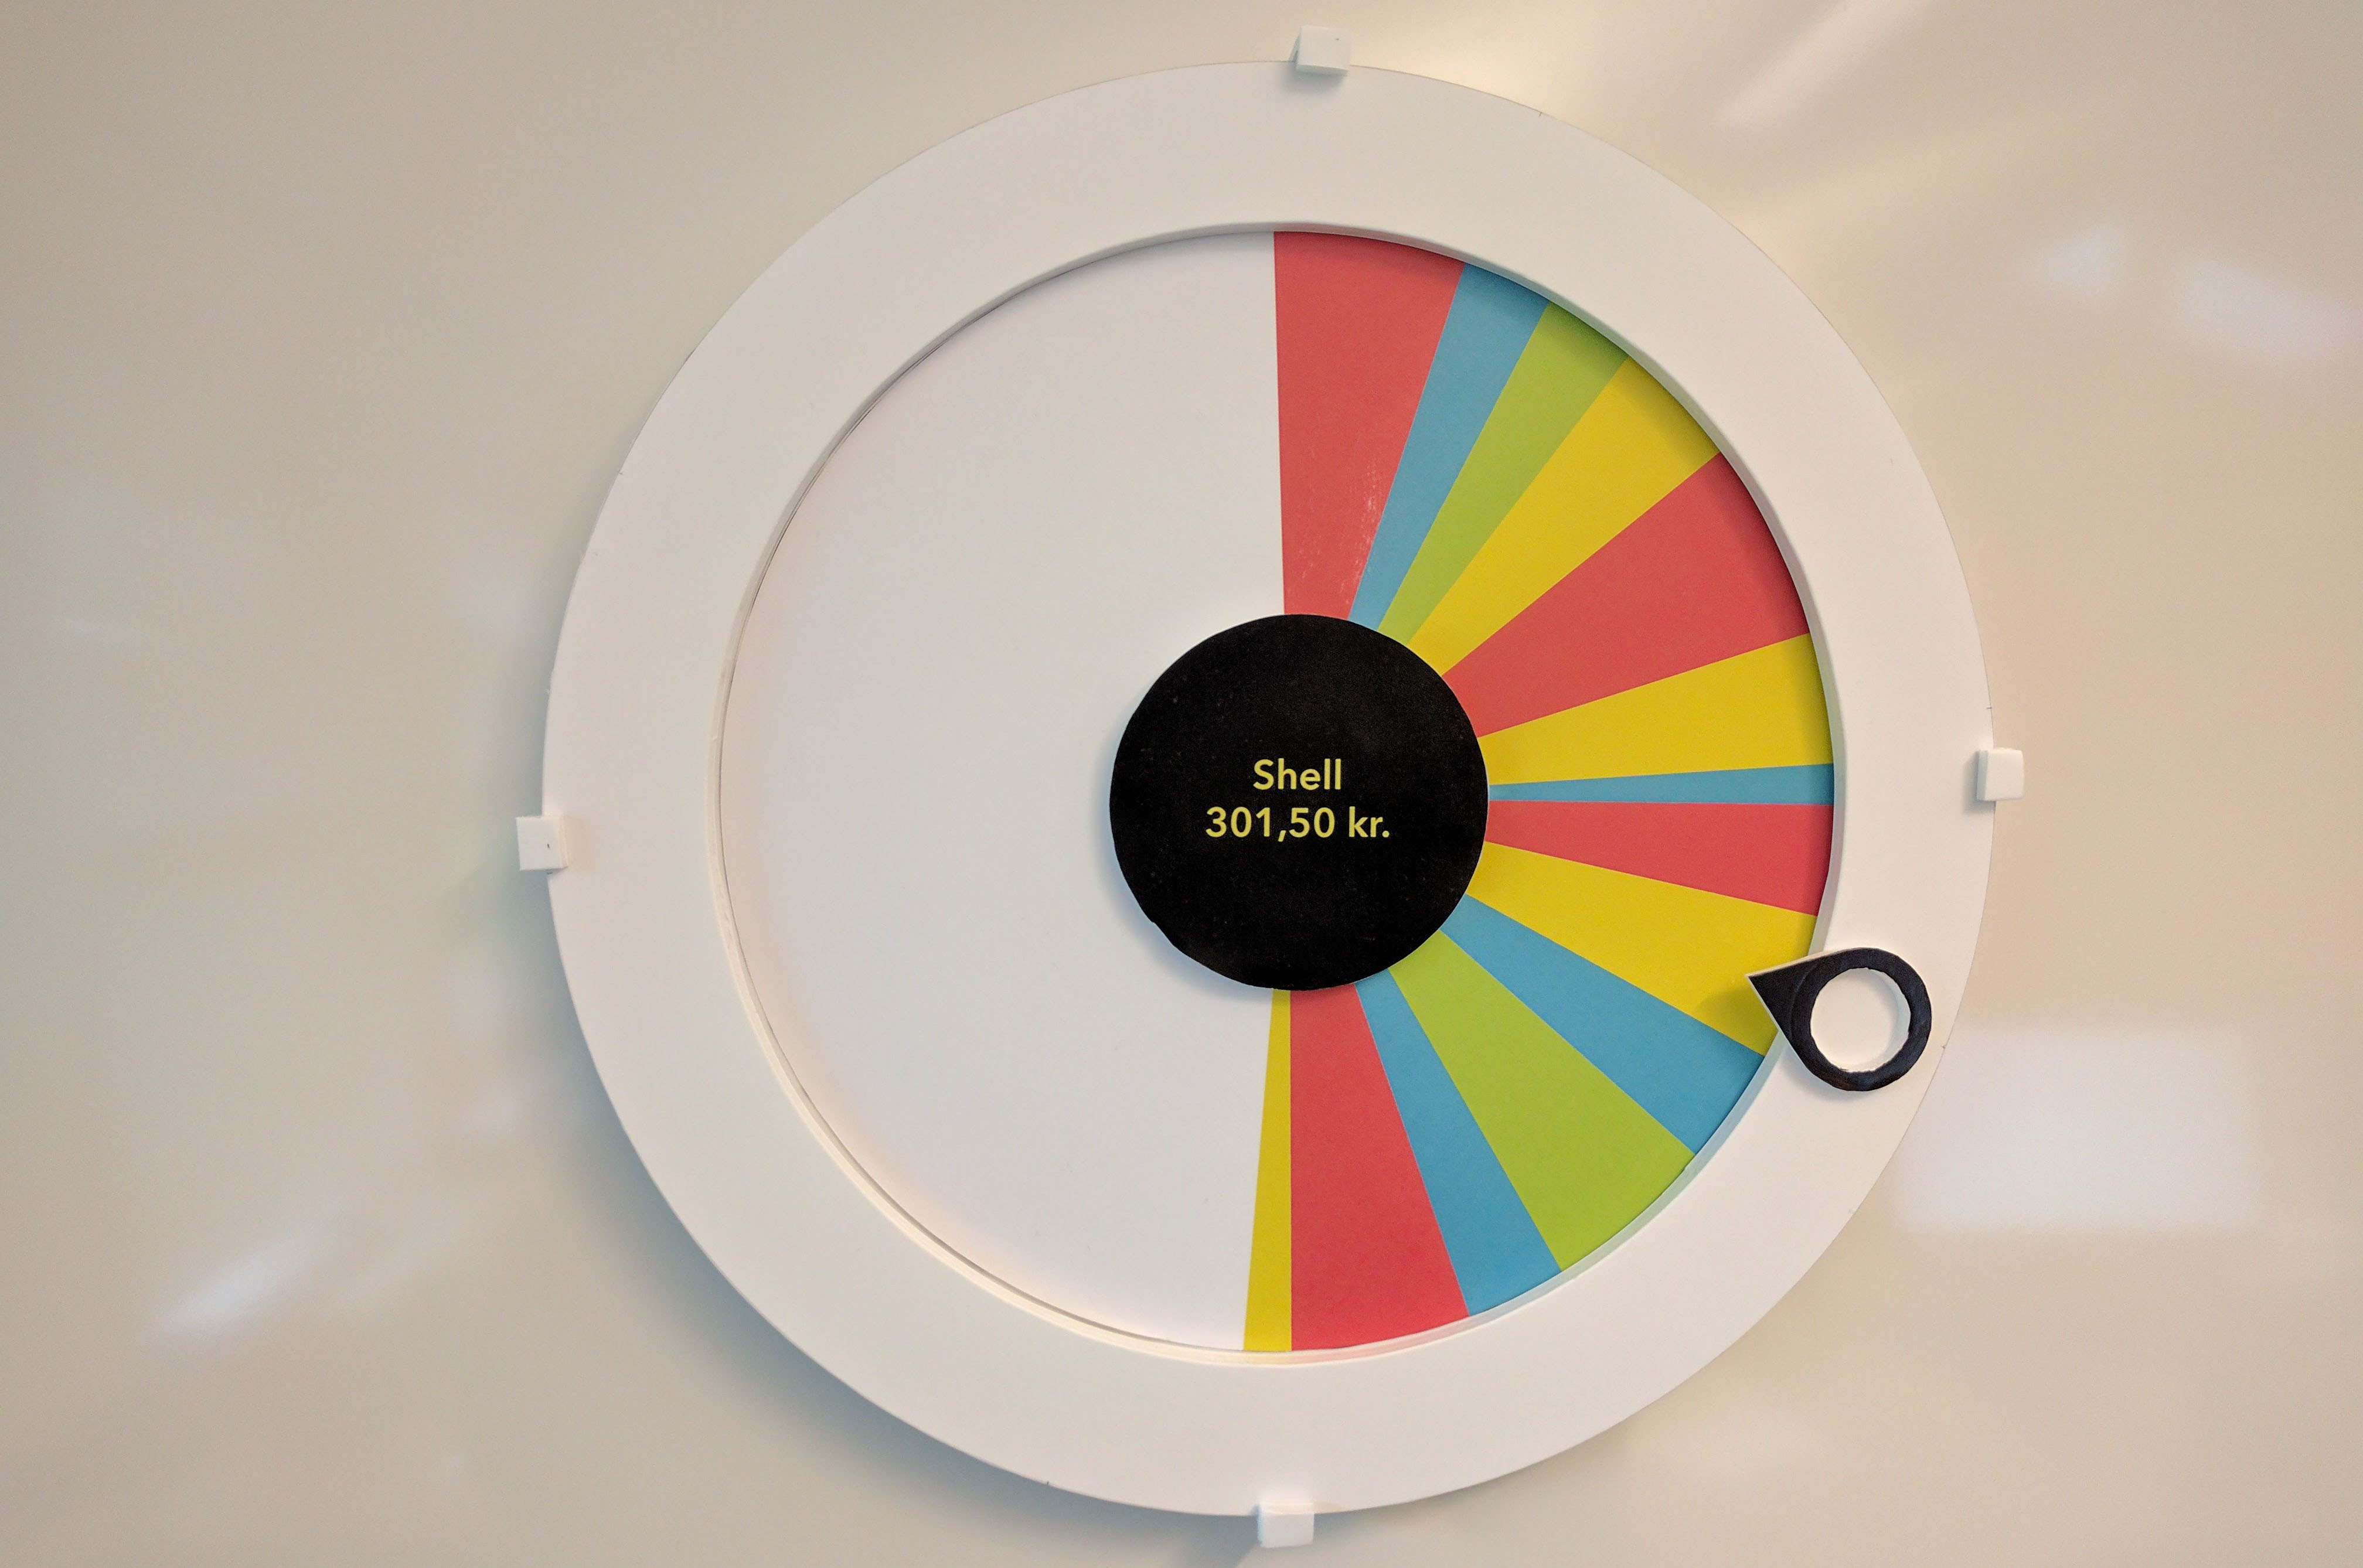
\includegraphics[width=0.75\textwidth]{financial-clock-low-fi}
	\caption{Financial Clock prototype enabling the user to get a monthly spending overview with indications of individual transactions that are inspectable by rotating the bezel of the clock}
	\label{fig:financial-clock-low-fi}
\end{figure}

\subsubsection*{Financial Speaker}
The Financial Speaker prototype (see figure figure~\ref{fig:financial-speaker}) is a small portable speaker that can be arranged and rearranged as the user wishes, which allows it to be easily integrated in existing activities and routines in the household. The Financial Speaker uses a speech interface to interact with the user along with sensing technology to infer the user’s presence. The prototype is configured through a smartphone application where the user chooses the financial information of interest and when to trigger it. For example, the Financial Speaker may be placed in the bathroom and configured to tell the user about relevant stock market information in the morning, when the user’s presence is inferred. The user may at any time ask the Financial Speaker to provide information on another economically related topic or stop playing, as is regular functionality of speech interfaces.

\begin{figure}[h]
	\centering
	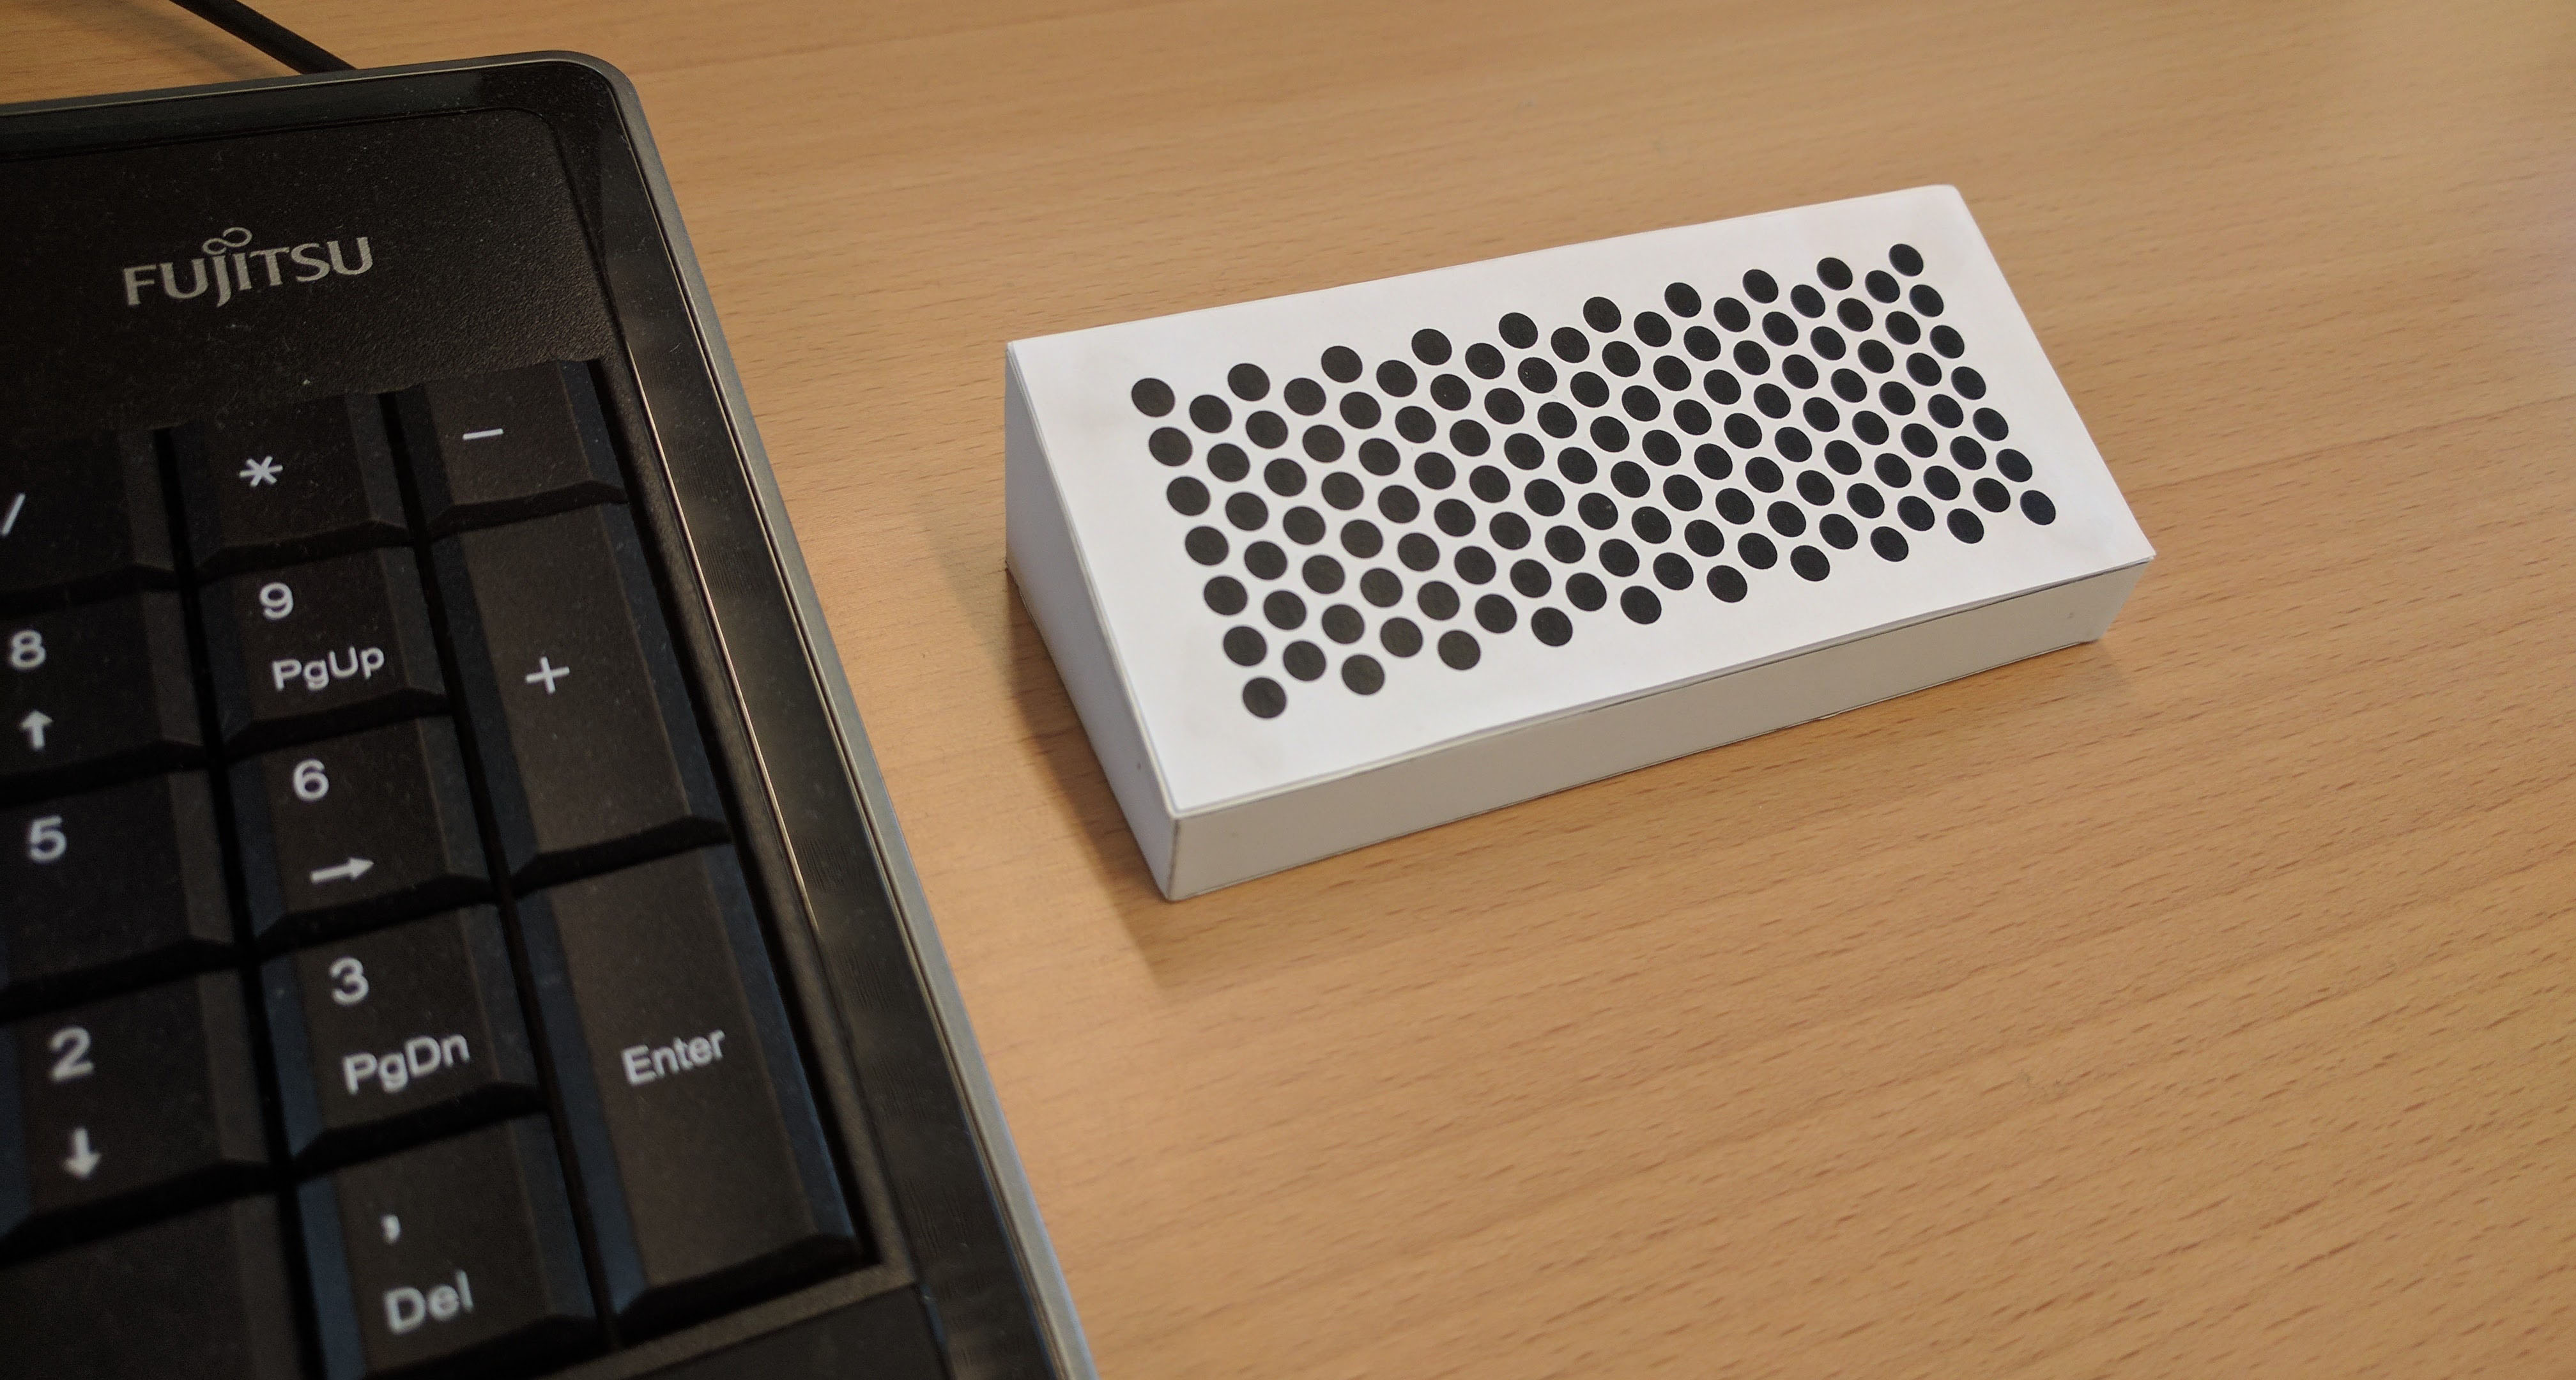
\includegraphics[width=0.75\textwidth]{financial-speaker}
	\caption{Financial Speaker prototype that features a speech interface and is able to communicate relevant financial information to the user based on smartphone configuration and placement in the home}
	\label{fig:financial-speaker}
\end{figure}

\subsubsection*{Evaluation of Initial Prototypes}
\label{sec:evaluation-of-initial-prototypes}
In order to assess the properties of the three prototypes we performed a small informal evaluation, lasting around 25 minutes, with three former workshop participants. As described earlier each prototype represents a specific focus and for this reason we, with this evaluation, sought to understand what features and/or qualities each prototype could bring to our final prototype. The ideas were presented one by one followed by a series of open question, e.g. “what do you think about the data representation?” and “how would you use such an object in your home?”.

When we presented the Coffee Mug concept to the participants they seemed to like the simplicity of it, yet they were not sure if they would use it on a daily basis. When asked about the data representation one of the participants responded \emph{“I think it is fine, because I don’t need a specific number to know how much [money] I have left]”}. Another participant pointed out that visualization of the data was, due the asymmetric shape of the handle, somewhat difficult to read and thus a bit ambiguous. Even though the data was showed in a low resolution format and presented relatively to a monthly budget, they did not like that information was visible to others. The second prototype we presented was the Financial Speaker. Compared to the Coffee Mug one of the participants liked that he had the initiative, meaning that he could seek out information and had some kind of control over the data. In his words emph{“the information doesn’t need to be present all the time”}. We asked the participants where they imagined to use such a product to which they responded in the bathroom, bedroom or office. One of the participants did not like the visual appearance of the speaker as he felt it looked too utilitarian. He told us that he considered buying the Google Home speaker (a voice-activated speaker created by Google) once it became available in Denmark because it resonates well with a home: \emph{“it looks like it belongs there”}. All the participants generally liked the third prototype, the Financial Clock, especially because it provided a good overview and an intuitive interaction. However, the participants argued over the look of the bezel with the black clock hand. Two of the participants really liked it whereas the third one did not because it reminded him of an old telephone. Presenting a monthly view made sense to the participants as one (usually) receives salary and bills once a month. One participant suggested to divide the dial into four parts as it would become easier to view one week at a time.

To summarise this short evaluation, it confirmed that abstract data representations are something to pursue and that privacy is a topical area within our domain. Furthermore, the evaluation underlined that interactive household objects should stylistically align with the home in order to establish a sense of belonging -- in other words, artifacts created for a home should be seamlessly integratable. Based on the feedback and our own designerly intuition we have chosen to work with the Financial Clock as it got great remarks from the participants while also presenting many possible design directions due to its relative complexity compared to the other ideas. Choosing this direction is an acknowledgement of the importance of context integration when designing domestic technology for personal financial management, as the Financial Clock prototype was centered around the emerging theme of seamless context integration. The decision to go in this particular direction has shaped our further design process as it provides the basis for our second research question: \emph{“How can we design interactive domestic technology for personal financial management that is seamlessly integrated into the home?”}. The following sections present our effort to answer this question through iterative prototype development.

\section{Prototyping}
This section presents our further work and iterations on the Financial Clock prototype. First, we present some design guidelines that act as important considerations for our design choices, followed by design work that has acted as an inspiration in the design process, especially in relation to data representation and aesthetics. Then, we go into detail with the iterations on the prototype and present our design choices based on relevant literature and terminology, among these the taxonomy of Ambient Information Systems. Lastly, we elaborate on the notion that we call Emergent Displays which we believe is a promising way for interactive domestic technology to become truly integrated in the home and to ensure the privacy of sensitive data in this context.

\subsection{Design Guidelines}
Going from broad idea generation into more focused prototyping and iteration on the Financial Clock concept, we find it useful to keep some design guidelines in mind as we concretize the concept further. The guidelines are gathered from our own findings and the presented literature and essentially describe the factors that we have found to be important in designing interactive domestic technology for personal financial management with a focus on seamless context integration. The guidelines are presented in the following list along with a short description:

\vspace{12pt}
\begin{itemize}
	\item\textbf{Aesthetics}: Emphasis on style and visual aesthetic. Artifacts designed with a high level of aesthetic emphasis have better opportunities to establish a sense of domestic belonging. Consequently, objects that are designed without attention to style and domestic properties have a lower chance to be integrated in the context.
	\item\textbf{Privacy}: The data should only be perceivable by the intended receiver and data should be protected from unauthorized persons.
	\item\textbf{Data Abstraction Level}: The level of data abstraction. Data embedded into and expressed through abstract shapes or structures has a high data abstraction level, whereas exact and detailed data has a low abstraction level.
	\item\textbf{Current Status}: The system should enable the user to view status; preferably glanceable (low effort).
	\item\textbf{Data Persistence}: The data persists over time in such a way that trends and overall progress are detectable -- this is comparable to Li et al.’s history category.
	\item\textbf{Data Inspectability}: The presented data should be inspectable to some degree, allowing the user to engage with the data (possibly in a serendipitous way).
\end{itemize}
\vspace{12pt}

These guidelines are not necessarily hard requirements that the prototype must meet but rather important considerations when we explore the design space further and make design choices as we move forward.

\subsection{Exploring the Prototype Dimensions}
In our exploration of the design space we use Lim et al.’s framework for prototype conceptualization, the anatomy of prototypes /cite{lim2008anatomy}. This essentially means thinking of prototyping as filtering specific qualities of design ideas and manifesting them in the simplest way possible without distorting the understanding of the whole.

The following sections describe our explorations and design choices regarding the Financial Clock prototype. Design activities that we find are logically related are gathered and presented in sections together. It is important to note that this does not represent the actual order in which the activities were carried out, as many activities in reality ran in parallel tracks and informed each other in numerous ways.

\subsubsection*{Seeking Inspiration}
As part of the design process we sought inspiration from various resources. Firstly, we found pictures online of elegant clock concepts and created a small collage out of them (see figure~\ref{fig:clock-collage}). What struck us the most about many of the clocks that we found interesting was their simplicity; both in terms of materials and of visual appearance. The vast majority of the clocks have a plain-colored clock face and express time in a very minimalistic manner. Three clocks that we found especially fascinating were Lash Clock by Bina Baitel, ETCH Clock by ETCH and STORY by Flyte \cite{lash-clock,etch-clock,story} -- each clock utilizes a unique technique to convey time. For instance, Lash Clock conveys time through a ring of fibres and the ETCH Clock uses vacuum to create concave numbers on a flat surface. STORY is a bit different as it has three different modes. Using a levitating iron ball to depict time STORY can work as a normal clock, be a timer or show a journey, which essentially is a countdown timer linked to a story such as “time to next marathon”.


\begin{figure}[h]
	\centering
	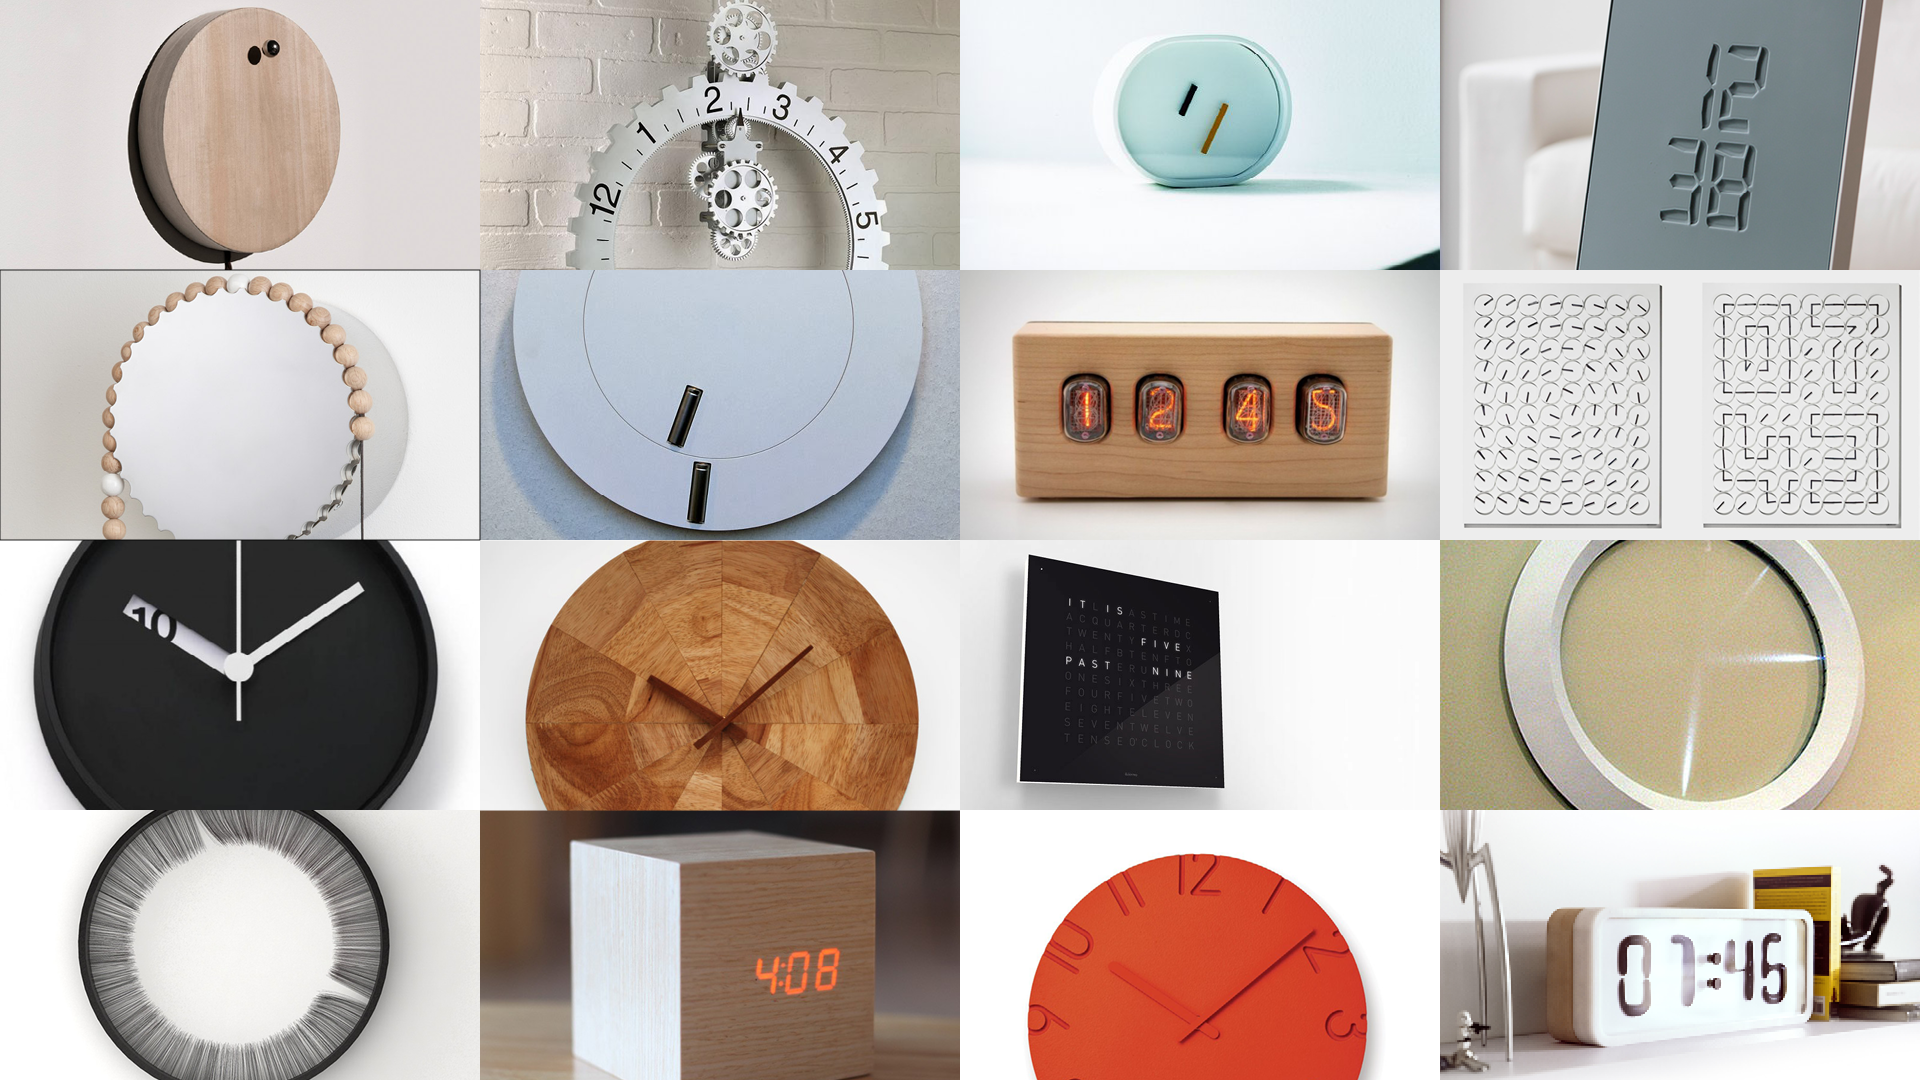
\includegraphics[width=0.9\textwidth]{clock-collage}
	\caption{Collage of different clocks}
	\label{fig:clock-collage}
\end{figure}

Secondly, based on online research as well as previously encountered art pieces/products, we investigated similar and compelling concepts within our design space -- some use the idea of a clock whereas others utilize an interesting technology. The Whereabouts Clock developed by Brown et al. \cite{brown2007locating} is a location awareness system for families. Using cell phone data the clock shows a symbolic location, such as “home” or “work”, for each individual family member. It aims to provide family members with reassurance, identity, connectedness and social touch. A more artistic clock is Last by Ängeslevä and Cooper \cite{angesleva2005last}. It uses 1-pixel vertical slices from a video feed and three concentric circles (one for hours, minutes, seconds) to represent time; as time passes the clock “paints” with the 1-pixel slices leaving a trail of what has happened in the past (in front of the camera). Another project that we found great inspiration in is HEART BLOOM, which was presented at the Dutch Design Week 2016. Using bio-data and a pen plotter a circular pattern created from heart information is plotted on a piece of paper -- the finished product looks a lot like a flower. This way of recording and presenting information we found very appealing. Lastly, BERG and Google made a project together were they augmented “dumb” objects by tracking and superimposing graphics onto them \cite{berg2011lamps}. The quality of light and the graphical freedom this kind of solution brings was also something we found very interesting.

\begin{figure}[h]
	\centering
	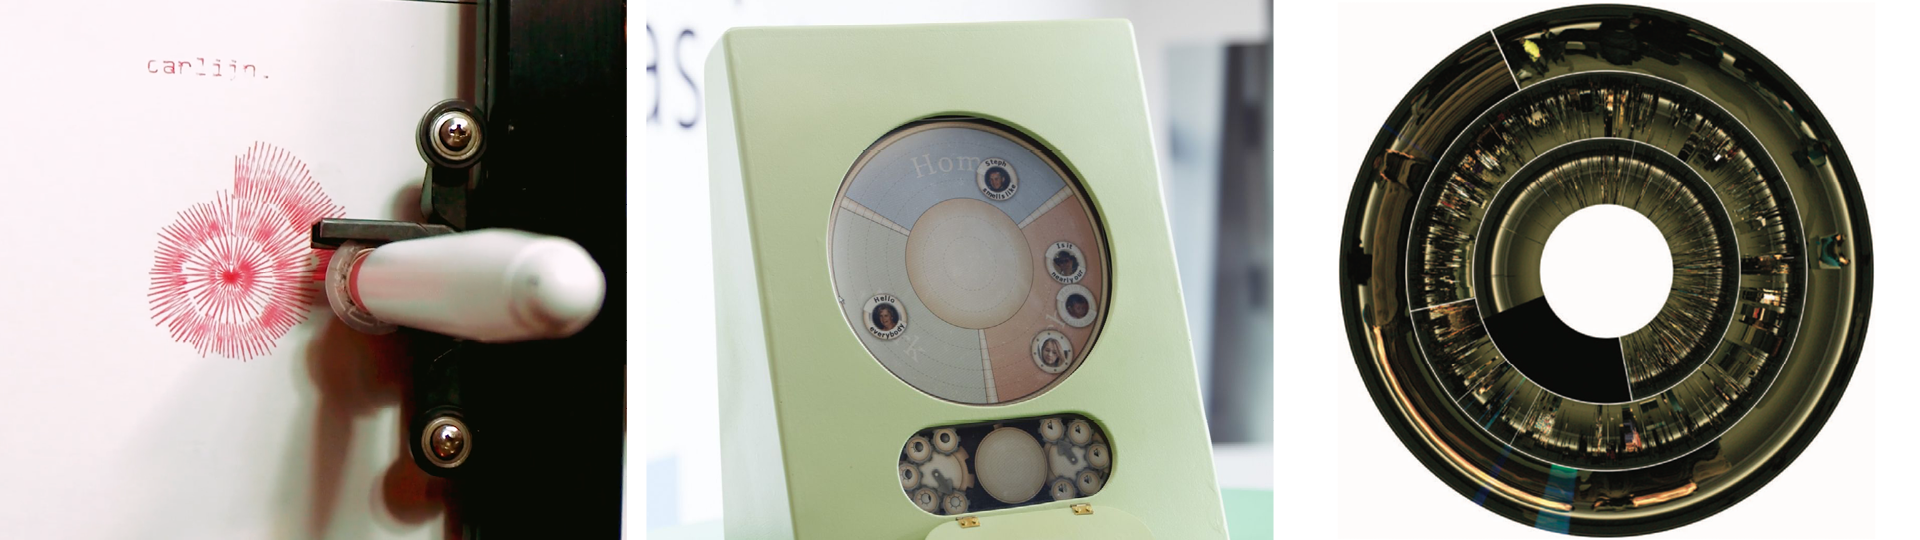
\includegraphics[width=0.95\textwidth]{heart-bloom-whereabouts-last}
	\caption{First: HEART BLOOM; Second: Whereabouts Clock; Thirds: Last Clock}
	\label{fig:heart-bloom-whereabouts-last}
\end{figure}

\subsubsection*{Refining the Financial Clock Concept}
\label{sec:refining-the-financial-clock-concept}
Based on the inspiration from the previous section, we set out to define the overall direction for the Financial Clock concept, i.e. taking a step back and looking critically at the concept as it is presented in the ideation section. We decided to broadly investigate many aspects of the Financial Clock concept, including, among others, the numerous ways in which the user’s financial data can be represented, interaction possibilities, physical form, and which technology to use as it has great implications on the opportunities and limitations regarding other aspects, such as interaction and data representation. We tried to be relatively open minded in exploring the possibilities of the Financial Clock concept, meaning that we did not explicitly use the design guidelines to constrain ourselves in the process but rather to analyze and evaluate the ideas iteratively.

The ideas presented in the following draw fundamental inspiration from AIS, specifically the idea that systems are able to reach out to the users and grab their attention in subtle ways instead of users having to actively seek out information.

Starting the exploration towards a concept with more explicit focus on seamless context integration we naturally took the Financial Clock concept presented in the ideation section (section~\ref{sec:financial-clock-concept}) as a point of departure. While the concept in its initial form was created based on the theme of seamless context integration, we find that guidelines such as aesthetics, privacy and data abstraction could be addressed to further emphasize the theme. To address these guidelines we generated a handful of ideas (see figure~\ref{fig:whiteboard-clock-ideas}). Many of these were intuitively focused on abstract data representations that were either symbolic or iconic in nature as these make it harder for unintended receivers to perceive the financial information that is being conveyed, thus increasing privacy. Additionally, abstract representations may be recognized as aesthetically pleasing. One idea focusing on abstract representation was to cast a shadow up on the wall which resembled an eclipse. The eclipse would then gradually move corresponding to the user’s spendings and thus act as a status overview. Ideas going in this direction move towards the Informative Art category where ideas become art with simple information embedded. While we find this direction intriguing due to the aesthetic emphasis and implicit respect for privacy caused by highly abstract data representations, there are still two guidelines left unattended; persistence and inspectability. Persistence is important because it enables the users to look for patterns in their long-term data while inspectability empower the users to engage with the data in more detail and look for discrepancies. Both of these guidelines are concerned with fostering self-reflection which is essential to our goal of increasing economic awareness, therefore they must be addressed.

\begin{figure}[h]
	\centering
	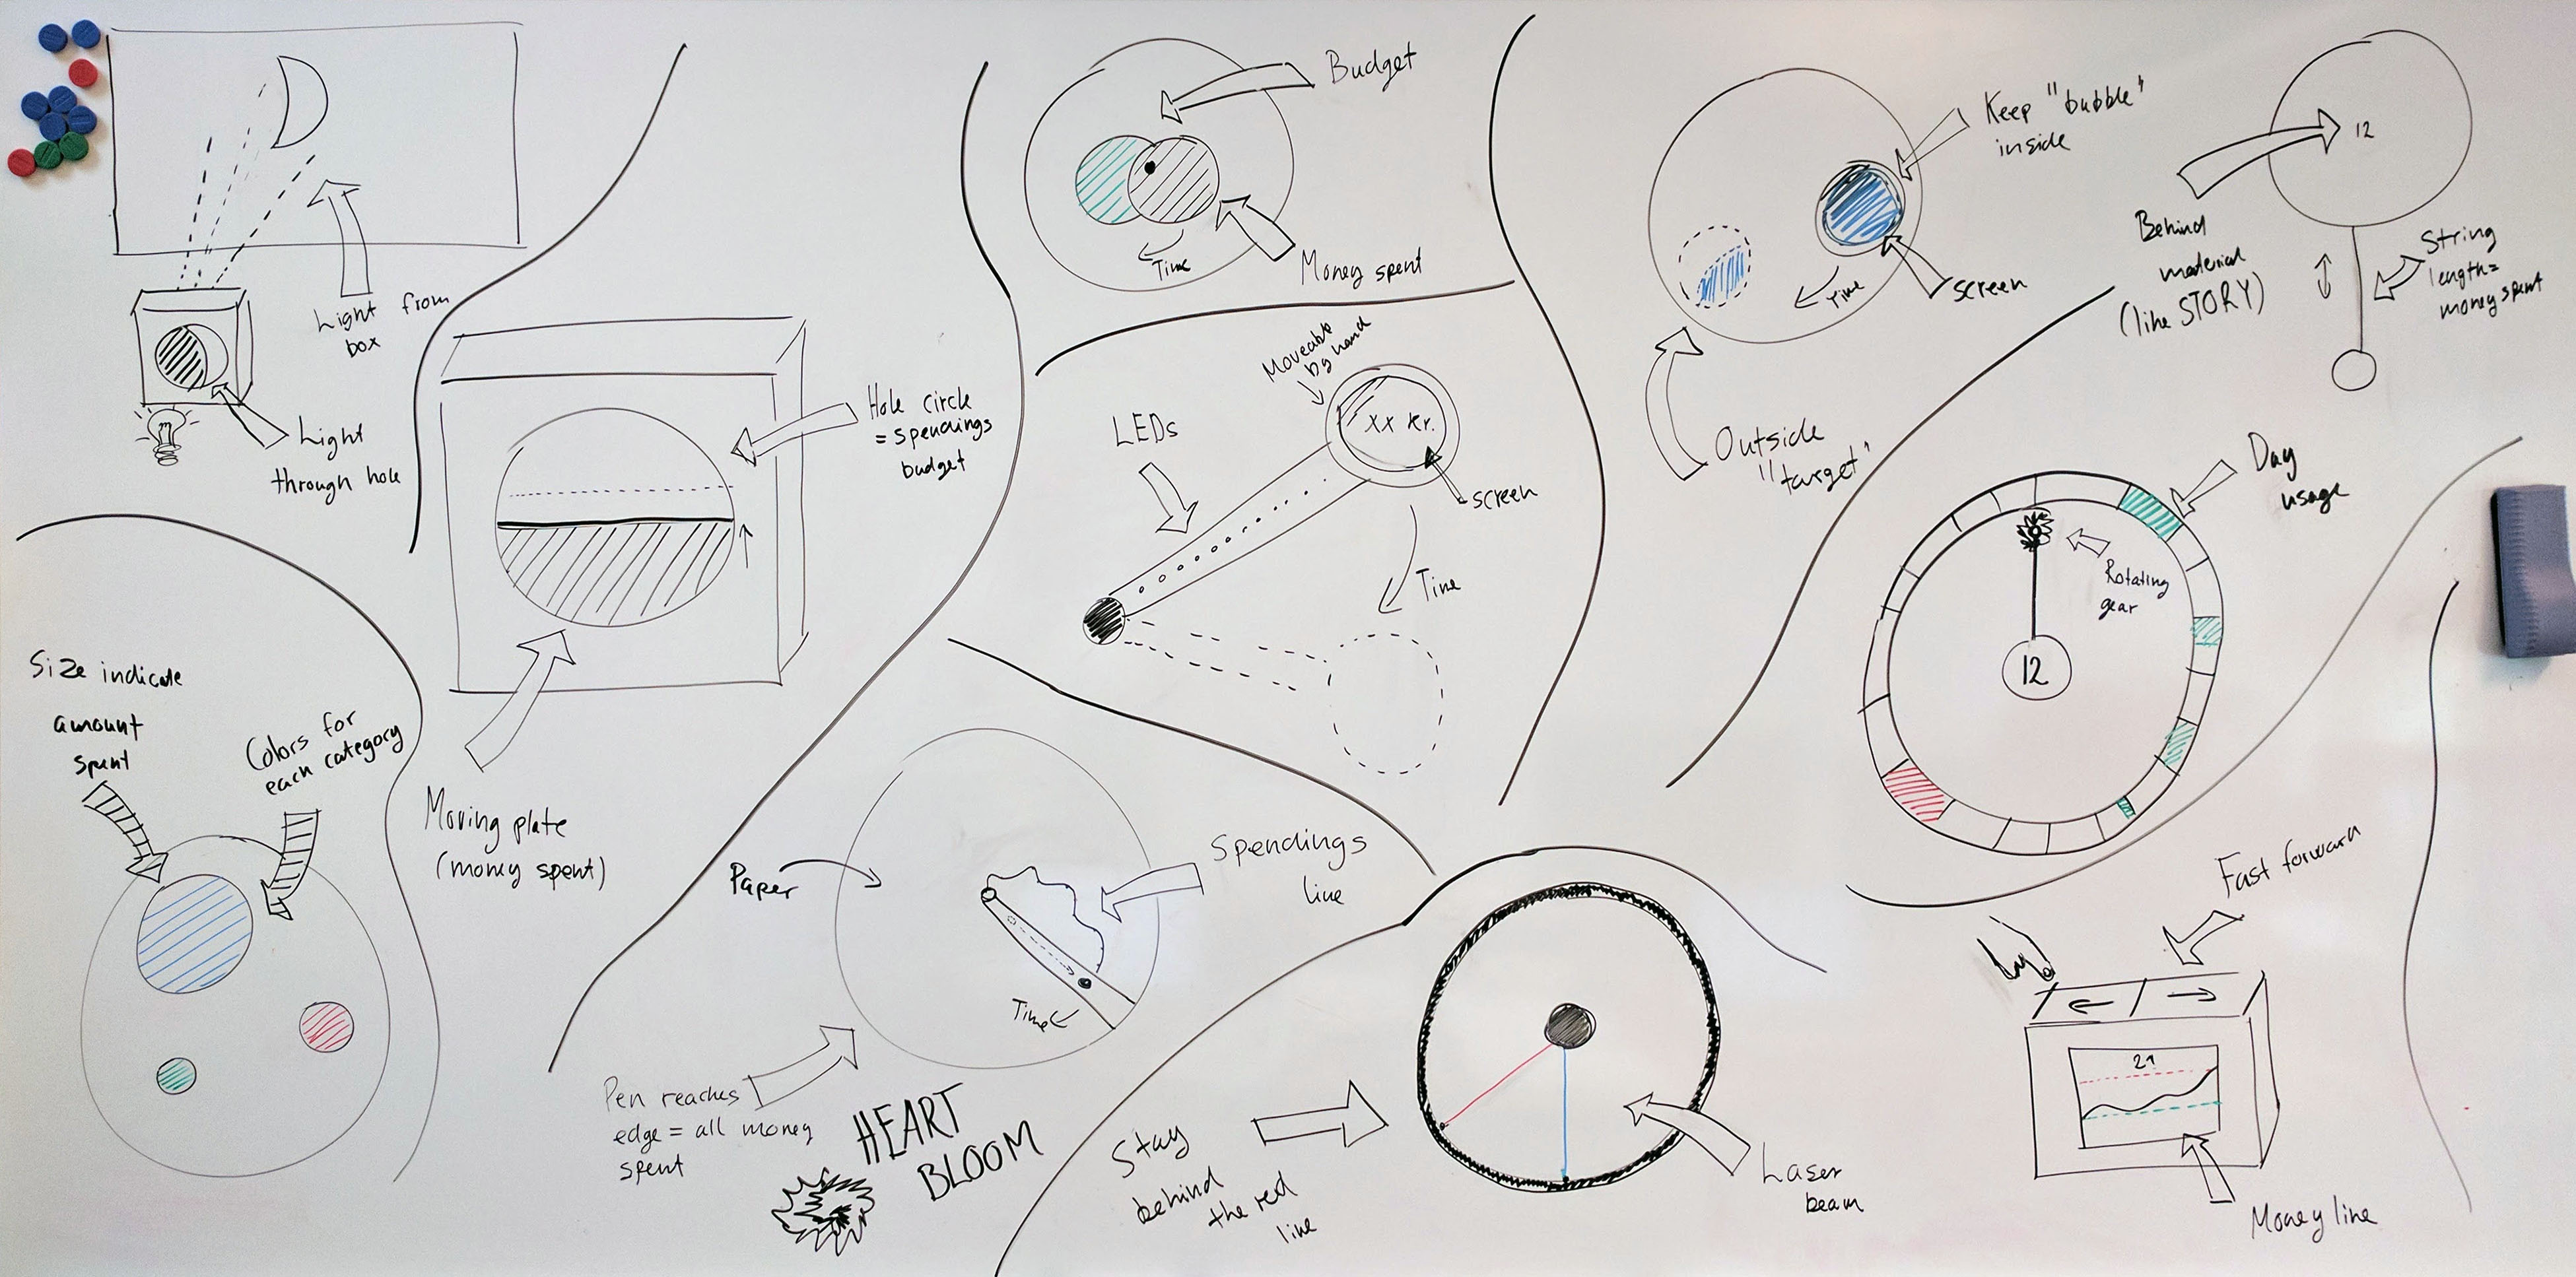
\includegraphics[width=\textwidth]{whiteboard-clock-ideas}
	\caption{Picture of whiteboard sketches that explore the possibilities of the Financial Clock concept}
	\label{fig:whiteboard-clock-ideas}
\end{figure}

One idea that provided data persistence was inspired by the HEART BLOOM project. The clock dial is covered with paper and the clock hand extends from the center to the bezel with a pencil attached to it. The pencil is able to move back and forth along the clock hand, creating a drawing that depicts the user’s spendings over the course of a month. This idea allows the user to reflect on the history of his spendings but still lacks the ability to inspect any of the information. This is a common tendency we found in our exploration, ideas that only utilize mechanical movement have a hard time creating dynamic representations, which is required to properly support the design guideline concerning inspectability. In order to accommodate this guideline we decided that some kind of dynamic display was necessary. We worked with the idea of incorporating a screen display in some concepts but felt like it was not entirely in line with the domestic aesthetics and our direction towards seamless context integration, as most people choose to install only a couple of screen-based objects in their homes, namely televisions and computers for the sake of leisure entertainment. We reckon that few people would like to have screen-based objects spread throughout their homes as they are associated with the efficiency of the workplace and as such does not comply with the aesthetics of the home. Instead, we sought inspiration in BERG and Google’s work on elegantly projecting graphics onto objects. What attracted us to pursue projection was the ability to retain the aesthetic properties of the object (e.g. shape and material) rather than sacrificing them for the utilitarian purposes of technology. This approach would allow us to design an aesthetic clock with a great sense of belonging in the home, however we still found that having a projected graphic on the clock all the time would be no less intrusive than having a screen-based object turned on all the time. Therefore, we decided to work with the notion of turning the display on/off based on sensing technologies such as proximity sensing, network activity or potentially even eye tracking. This particular idea gave rise to the concept we call Emergent Displays; displays that are able to emerge and augment household objects with information at moments when it is relevant to the user. The concept of Emergent Displays will be elaborated in a following section.
Taking the direction of turning the display on at appropriate times implies that it will be in the off state most of the time as not to constantly interfere with the user’s daily life. We believe it is important, especially in the case of a clock, that the designed object is meaningful in this off state in order to achieve a truly seamless integration in the home. Consequently, we decided that the Financial Clock should function as a regular clock in this off state. Essentially this means that the Financial Clock is able to switch between being a regular clock and a device for financial overview and inspection.

Summarising the Financial Clock concept after this exploration, we went in the direction of a multi-purpose device that can switch between regular clock and financial functionality in order to achieve a seamless integration in the home. Regarding the representation of the financial data, we found the idea of a drawing-like graphic that depicts the user’s monthly spendings interesting to pursue. Lastly, we believe that the form and interaction of the initial Financial Clock idea is worth keeping as the circular form elegantly affords the rotation interaction -- the interaction naturally arises from the form, offering a novel interaction experience with a clock.

\subsubsection*{Clock Design}
Now, with a more well-defined concept it is possible to “dissect” and explore the various design dimensions within our concept in a more focused manner. In this subsection we are going to present various investigations that we carried out in order to concretize the concept even further. In particular, we are going to use Lim et al.’s filtering dimensions, i.e. appearance, data, functionality, interactivity and spatial structure \cite{lim2008anatomy}, as a means to answer questions such as “what kinds of material are suitable for projected light?” and “how should the user be able to engage with the application content?”. Furthermore, we are going to use previously presented findings and literature as guiding principles in order to refine different aspects of the concept.

\begin{figure}[h]
	\centering
	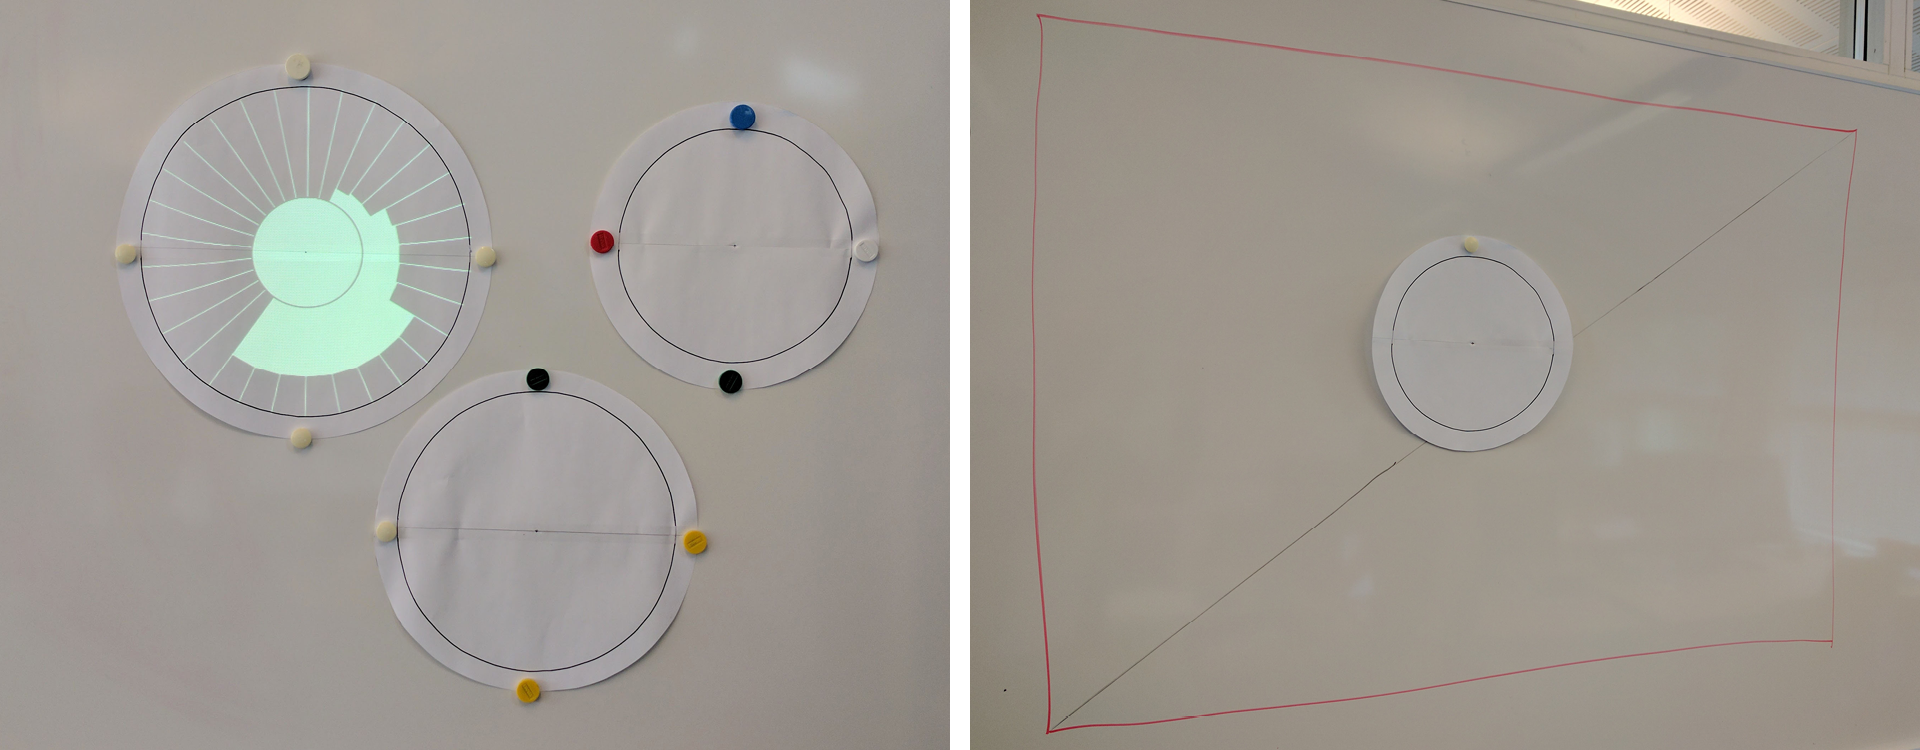
\includegraphics[width=\textwidth]{clock-size-exploration}
	\caption{Exploration of the clock size}
	\label{fig:clock-size-exploration}
\end{figure}

Having settled on the overall shape of the product (round like most wall clocks) our exploration into appearance began. In order to find a germane size for the clock face, we created a number of simple prototypes (see figure~\ref{fig:clock-size-exploration}). The prototypes were manifested in paper, with a low resolution and small scope \cite[p.~11]{lim2008anatomy}. The purpose of the clock size exploration was twofold; firstly we wanted to find a fitting size proportional to an average-size room and, secondly, as the size of clock face is equal to the dimensions of the interface surface  -- unless the wall around the clock is taking into use -- the size of the clock face will have an impact on the information density. Therefore, choosing a suitable clock size is important in order to avoid a grainy and/or distorted picture. Our material exploration is very much based on BERG’s video\footnote{\url{https://vimeo.com/55536920}} about projection materials. They mainly investigated how white light behaves on different types of wood, thus we extended this experiment by using colored light on a wider range of materials (see figure~\ref{fig:materials-light-exploration}). Perhaps not surprisingly, we found that in order to achieve an accurate graphical representation materials should be able to “absorb” light well. Also, when using colored light on dark/colorful materials, the colors of the light seem to be slightly distorted and less vibrant than on brighter materials. Consequently, we ended up using a somewhat light type of wood as we intended to represent current status through colors. For our last exploration into appearance we created an outline in Adobe Illustrator to iterate on the hour hand and the 3, 6, 9 and 12 markers. We decided to add the markers to the bezel due to earlier feedback (see section~\ref{sec:evaluation-of-initial-prototypes}) but also to accommodate for the new clock functionality.

\begin{figure}[h]
	\centering
	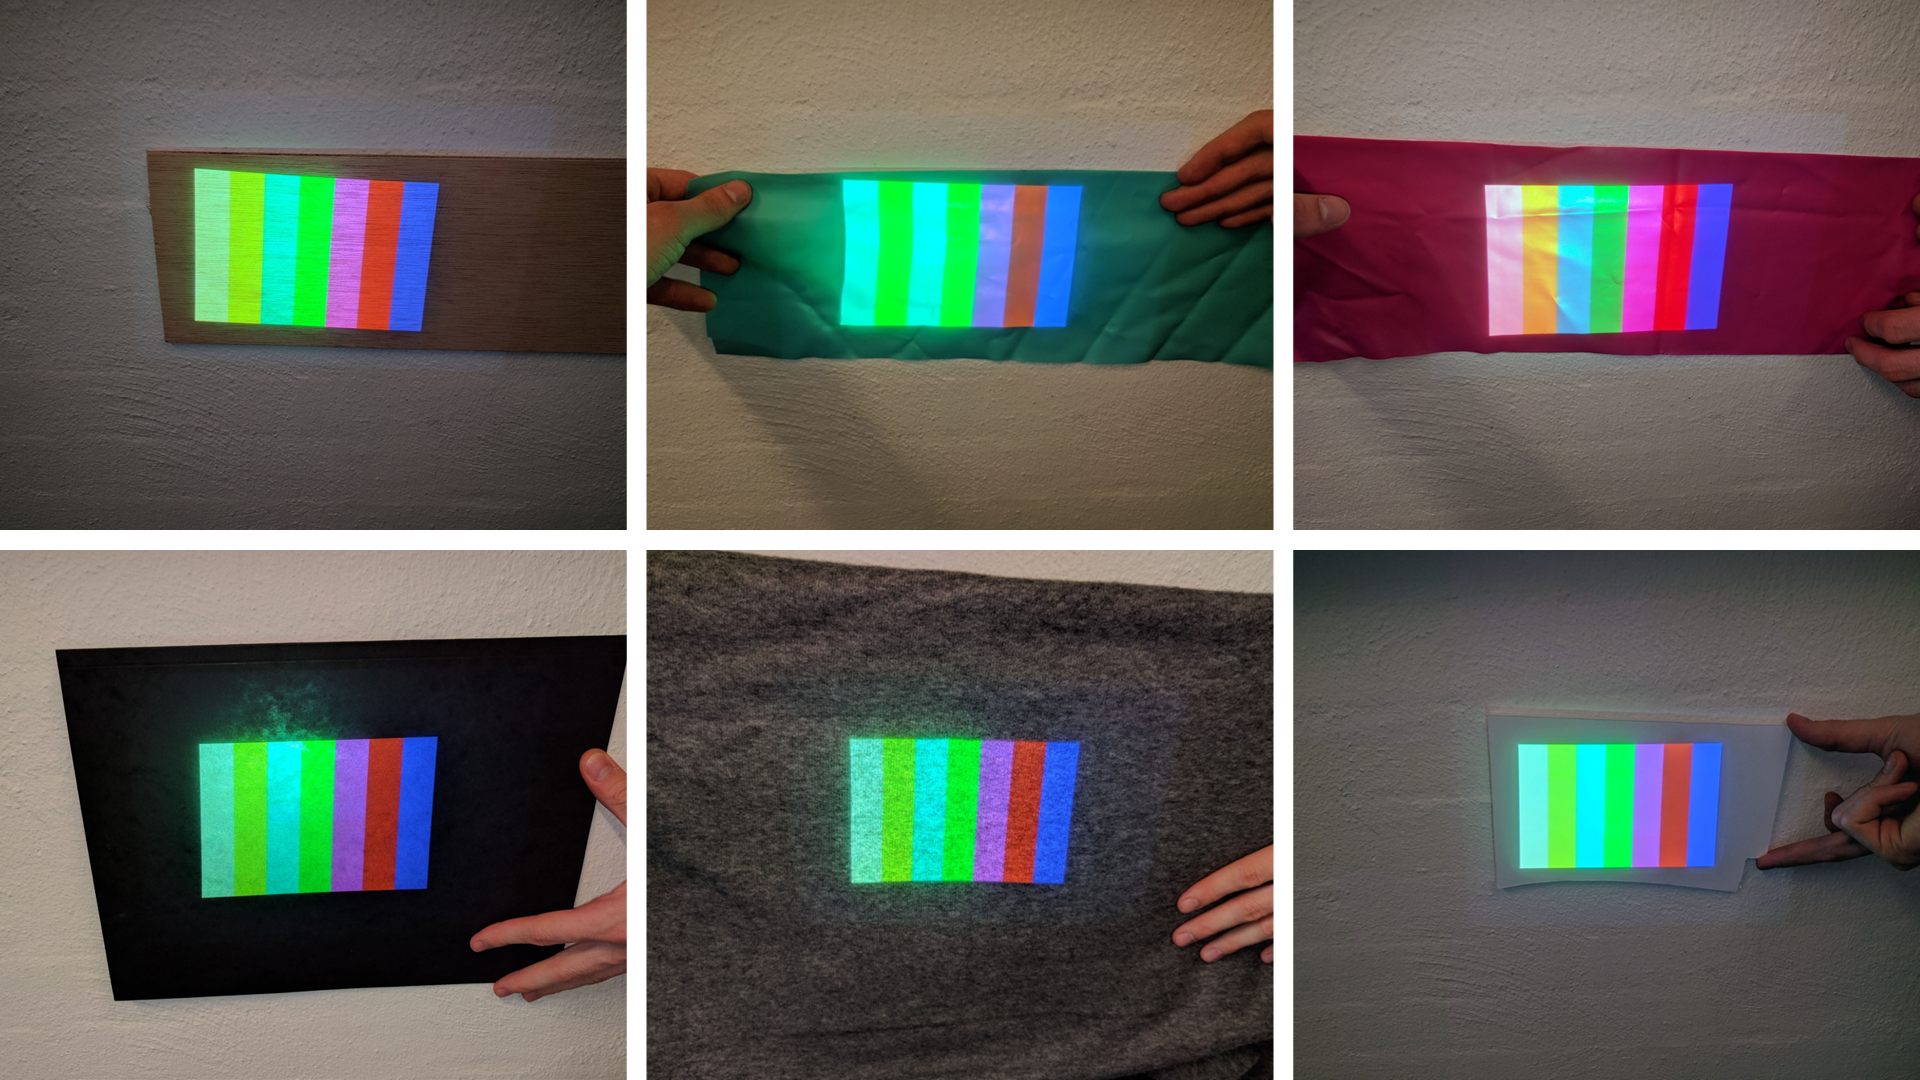
\includegraphics[width=\textwidth]{materials-light-exploration}
	\caption{Exploration of different materials}
	\label{fig:materials-light-exploration}
\end{figure}

In order to explore the inner workings of the prototype, i.e. the hardware and physical mechanisms, we created a prototype in foamcore (see the first and second image on figure~\ref{fig:foamcore-model-components}). As we intended to investigate the functionality in detail we tried to keep the resolution high and the scope relatively narrow. We rather quickly decided to use a stepper motor for the rotating mechanism since this would yield, as opposed to a servo motor or DC motor, a high accuracy and a low noise level. As a result our design revolved around the dimensions and properties of a regular stepper motor. During our investigation we found that many of the mechanisms in our design rely on high precision and the foamcore prototype highlighted that we need to include some clearance (i.e. some distance between two moving parts) in our final design in order to achieve a functional fit. In relation to the interaction (moving the clock hand), one of the features that we really liked as designers about our initial prototype (figure~\ref{fig:financial-clock-low-fi}) -- and found to be a controversial topic among the people who evaluated it -- was the physical manipulation of the bezel to “set time”. Even though we were very keen on this element we had to sacrifice it in order to preserve more indispensable features such as having a simple inner mechanics. For this reason we opted for an uncomplicated solution and ended up investigating alternatives. For instance, we enacted how various mechanisms from different standard hardware components (see third image on figure~\ref{fig:foamcore-model-components}) would work in relation to the movement of the clock hand. One of the more appealing solutions was the rotation (found on for example a potentiometer and a rotary encoder) since it has a natural mapping to the ration of the clock hand while being reminiscent of a crown found on regular wrist watches. However, unlike wrist watches there is no mechanical connection between the clock and the component meaning that the interaction could end up being perceived as disconnected and unresponsive. None of the other components offered something worth pursuing, so we chose the “easiest” solution, that is two buttons to control clockwise and counterclockwise rotation.

\begin{figure}[h]
	\centering
	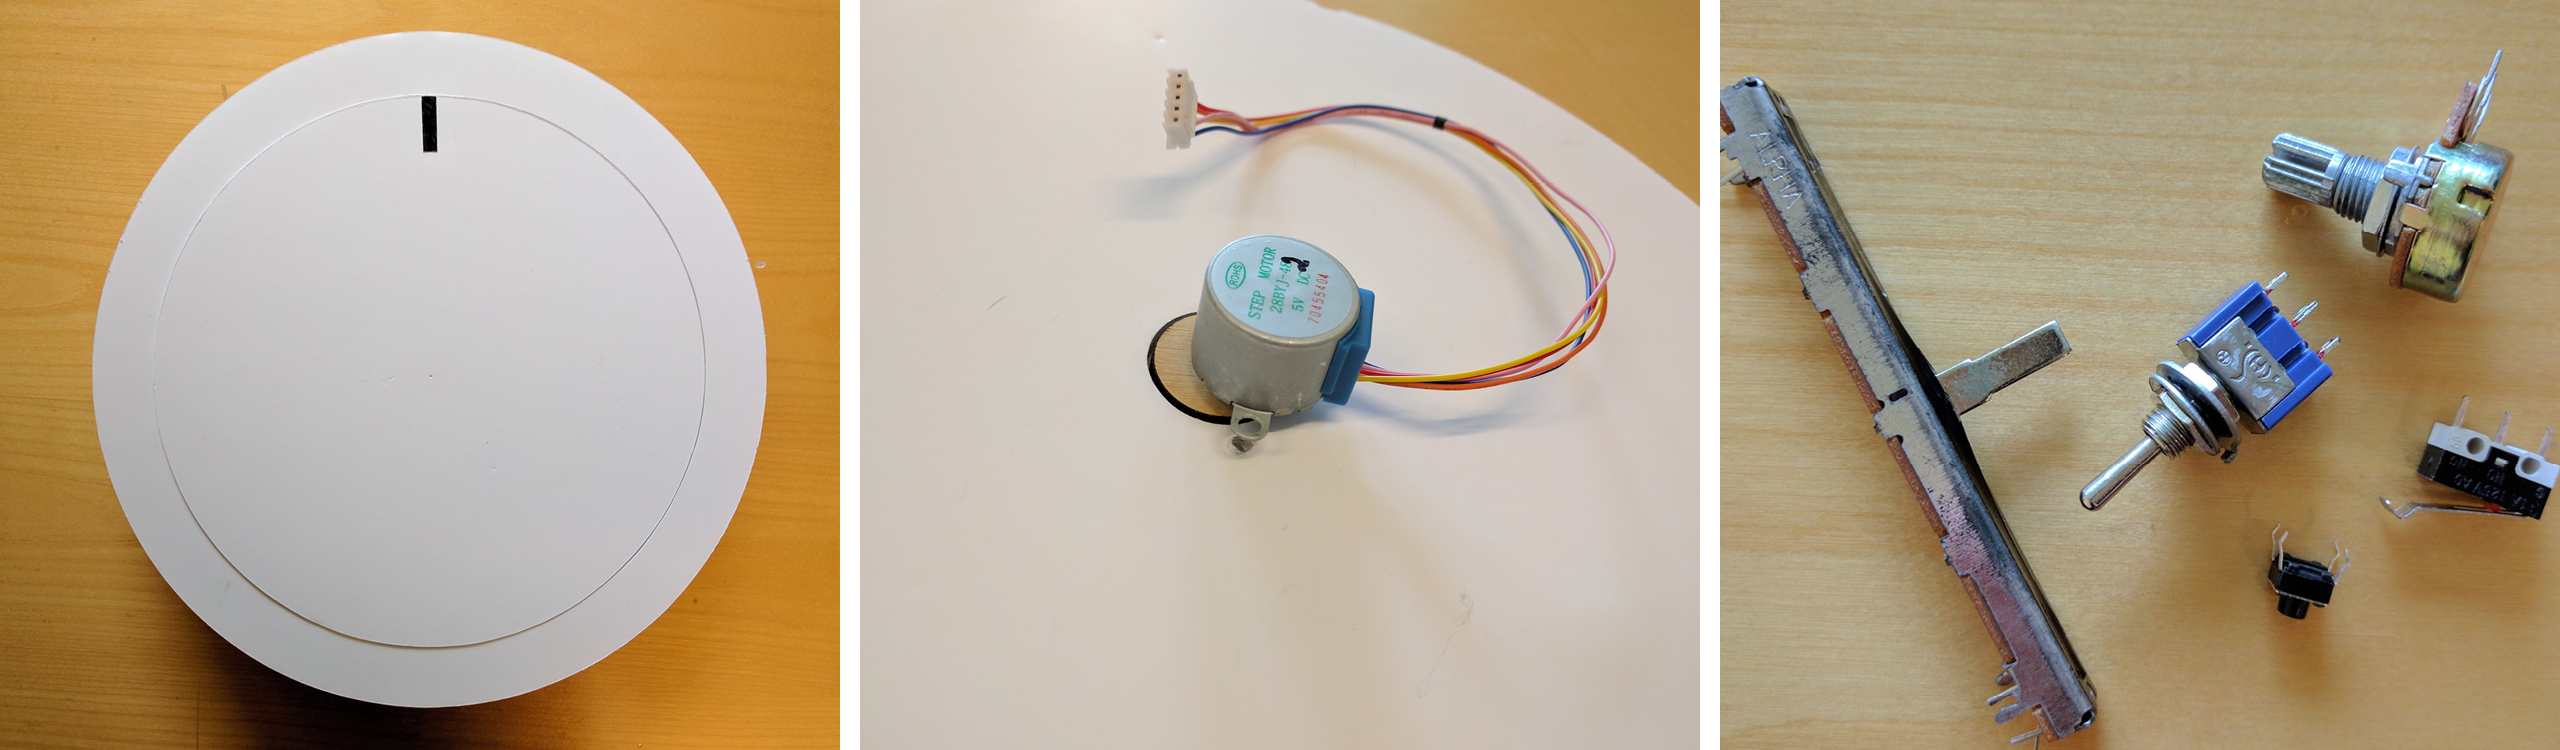
\includegraphics[width=\textwidth]{foamcore-model-components}
	\caption{Foamcore model and components}
	\label{fig:foamcore-model-components}
\end{figure}

Besides all the above-mentioned iterations, we had numerous iterations on the graphics and code, e.g. how to do projection mapping, how to correct keystone, color schemes for the graphics, etc. We are not going describe this in further detail, however some of the exploration into these aspects can be found on figure~\ref{fig:misc-exploration}.

\section{Emergent Displays}
As described in section~\ref{sec:refining-the-financial-clock-concept} our work with the Financial Clock concept led to an interesting combination of technologies, specifically projection mapping and internet-connected household objects, and we believe this combination can make for remarkable interaction experiences. Before we define the notion of Emergent Display we first need to establish a basis for it. We will start with a quote from Weiser and Brown on ubiquitous computing \cite[p.~5]{weiser1997coming}:

\tquote{It is easy to find 40 microprocessors in a middle class home in the U.S.A. today. They will be found in the alarm clocks, the microwave oven, the TV remote controls, the stereo and TV system, the kid’s toys, etc.\ldots Tie them to the Internet, and now you have connected together millions of information sources with hundreds of information delivery systems in your house}{Weiser and Brown, 1996}

With such a reality new opportunities for systems arise. Being connected to the internet devices are not only able to fetch data like software updates, weather information or tasty recipes, they can also interface with other devices and by that be used to compose comprehensive systems consisting of multiple devices. For such a vision to be attainable devices must implement and expose a uniform interface to the “public”, making it possible for other applications (running on other devices) to make use of their resources, e.g. sensor data like light, temperature and orientation or output components like LEDs, servo motors and speakers. One way to achieve this universal interaction architecture is by creating applications with RESTful APIs \cite{guinard2011internet}. This way of developing technology is going to be the technological bedrock for Emergent Displays -- if domestic household objects make it possible for other applications to make use of their resources, new layers of technology can be added.

At its core Emergent Displays can be described as ephemeral displays that emerge on top of and/or around internet-connected artifacts making use of their interactional features to apply secondary functionality. They are based on agile information carriers, such as shape change or projection mapping, meaning that a layer of information, i.e. the display itself, can dynamically emerge and disappear. For this reason Emergent Displays can be used to augment and enhance the expression of internet-connected objects while preserving their aesthetics qualities. In the context of Emergent Displays the meaning of ‘display’ refers to the temporary manifestation of information that once removed leaves the augmented object completely “untouched”. As described in the paragraph above the object being augmented should provide a set of interface “hooks” which secondary applications can make use of. For instance, a sunrise application can use events from an alarm clock to support and enrich the waking up experience or a countdown timer can be added to a toaster to show time left. An essential element in an Emergent Display is that once the information layer is added it should behave like an inherent part of the object, thus the coupling between changes in the emergent content and interaction needs to be tight. Also, applications utilizing this type of display should respect the physical properties and limitations of the augmented artifact. An underlying assumption about Emergent Displays is that the augmented object should make sense in all states, i.e. the object should be able to serve its original purpose and make sense while being augmented. One of the big questions when using this type of display is when the information layer should occur. One approach would be to use the resources (sensors for light, distance, temperature, etc.) from the augmented object, however it would also be possible to use resources from other devices/systems (security camera, door bell, etc.).

It is apparent that the domain of Emergent Displays is closely related to the research domain of AIS as it is inspired by the same vision of calm and environmentally integrated technologies which can enter the center of the user’s attention when needed and otherwise stay in the background. Emergent Displays and AIS share some fundamental behavioral characteristics such as a focus on representations \emph{in the environment} that are \emph{aesthetically pleasing} and environmentally appropriate. However, they deviate on \emph{when} the information, that the systems convey, is present in the environment. In AIS information is always present (ambient) with subtle changes that afford opportunistic glances. An Emergent Display on the other hand only presents the information when it is deemed necessary or appropriate, which we have argued may give a greater sense of belonging in the context. Considering the character of the data we believe that Emergent Displays may be useful to address information of greater importance/sensitivity (such as financial data) since the information is displayed on the terms of the users and otherwise hidden. Another significant difference is the focus on interaction with the information in our notion of Emergent Displays, which may provide a deeper level reflection about the data -- AIS is primarily concerned with conveying information. The obvious current challenge for Emergent Displays is the dependence on sensing technologies to infer when the display should emerge and disappear. However, we strongly believe the challenge will diminish as more UbiComp technologies appear and together will be able to infer more complex behavioral patterns. Even though sensing technologies may be a challenge they also provide the opportunity for users to configure and arrange when and under which circumstances the display should emerge.

\section{Final Prototype}
This section briefly summarises the developed Financial Clock concept that is the outcome of the exploration described in the Prototyping section and then presents the technical implementation of the concept.

\subsection{The Final Prototype Concept}
The Financial Clock looks like a regular round wall clock with a simplistic design in wood that arguably fits into a broad range of people’s homes (see figure figure~\ref{fig:final-prototype}). While functioning as a regular clock most of the time, it will react to the user’s proximity upon which a display of the user’s monthly spendings emerges on the dial. This spending graphic consists of a line that moves clockwise around the clock as the days pass (one revolution corresponding to one month) and towards the bezel as money are spent. The spending graphic is colored in nuances of green, yellow and red depending on the spendings and the user’s budget, with green meaning that the current spendings are on track with the budget and red indicating overspending. Spendings on any particular day can be inspected using a controller device, that rotates the dial, placed just below the clock. When rotating the dial with the controller device, the clock hand acts as an indicator showing which day is being inspected with the corresponding transactions displayed in the center of the dial. If multiple transactions are present on the same day, they will be shown one at a time using a smooth fade animation. Once the user stops interacting with the clock and leaves, it will rotate the dial, and thus the clock hand, back to the position indicating time of the day and turn the display off returning to the state of a regular wall clock.

A video showcasing the implemented prototype can be found at the following link: LINK

\subsection{Technical Implementation}

\begin{figure}[h]
	\centering
	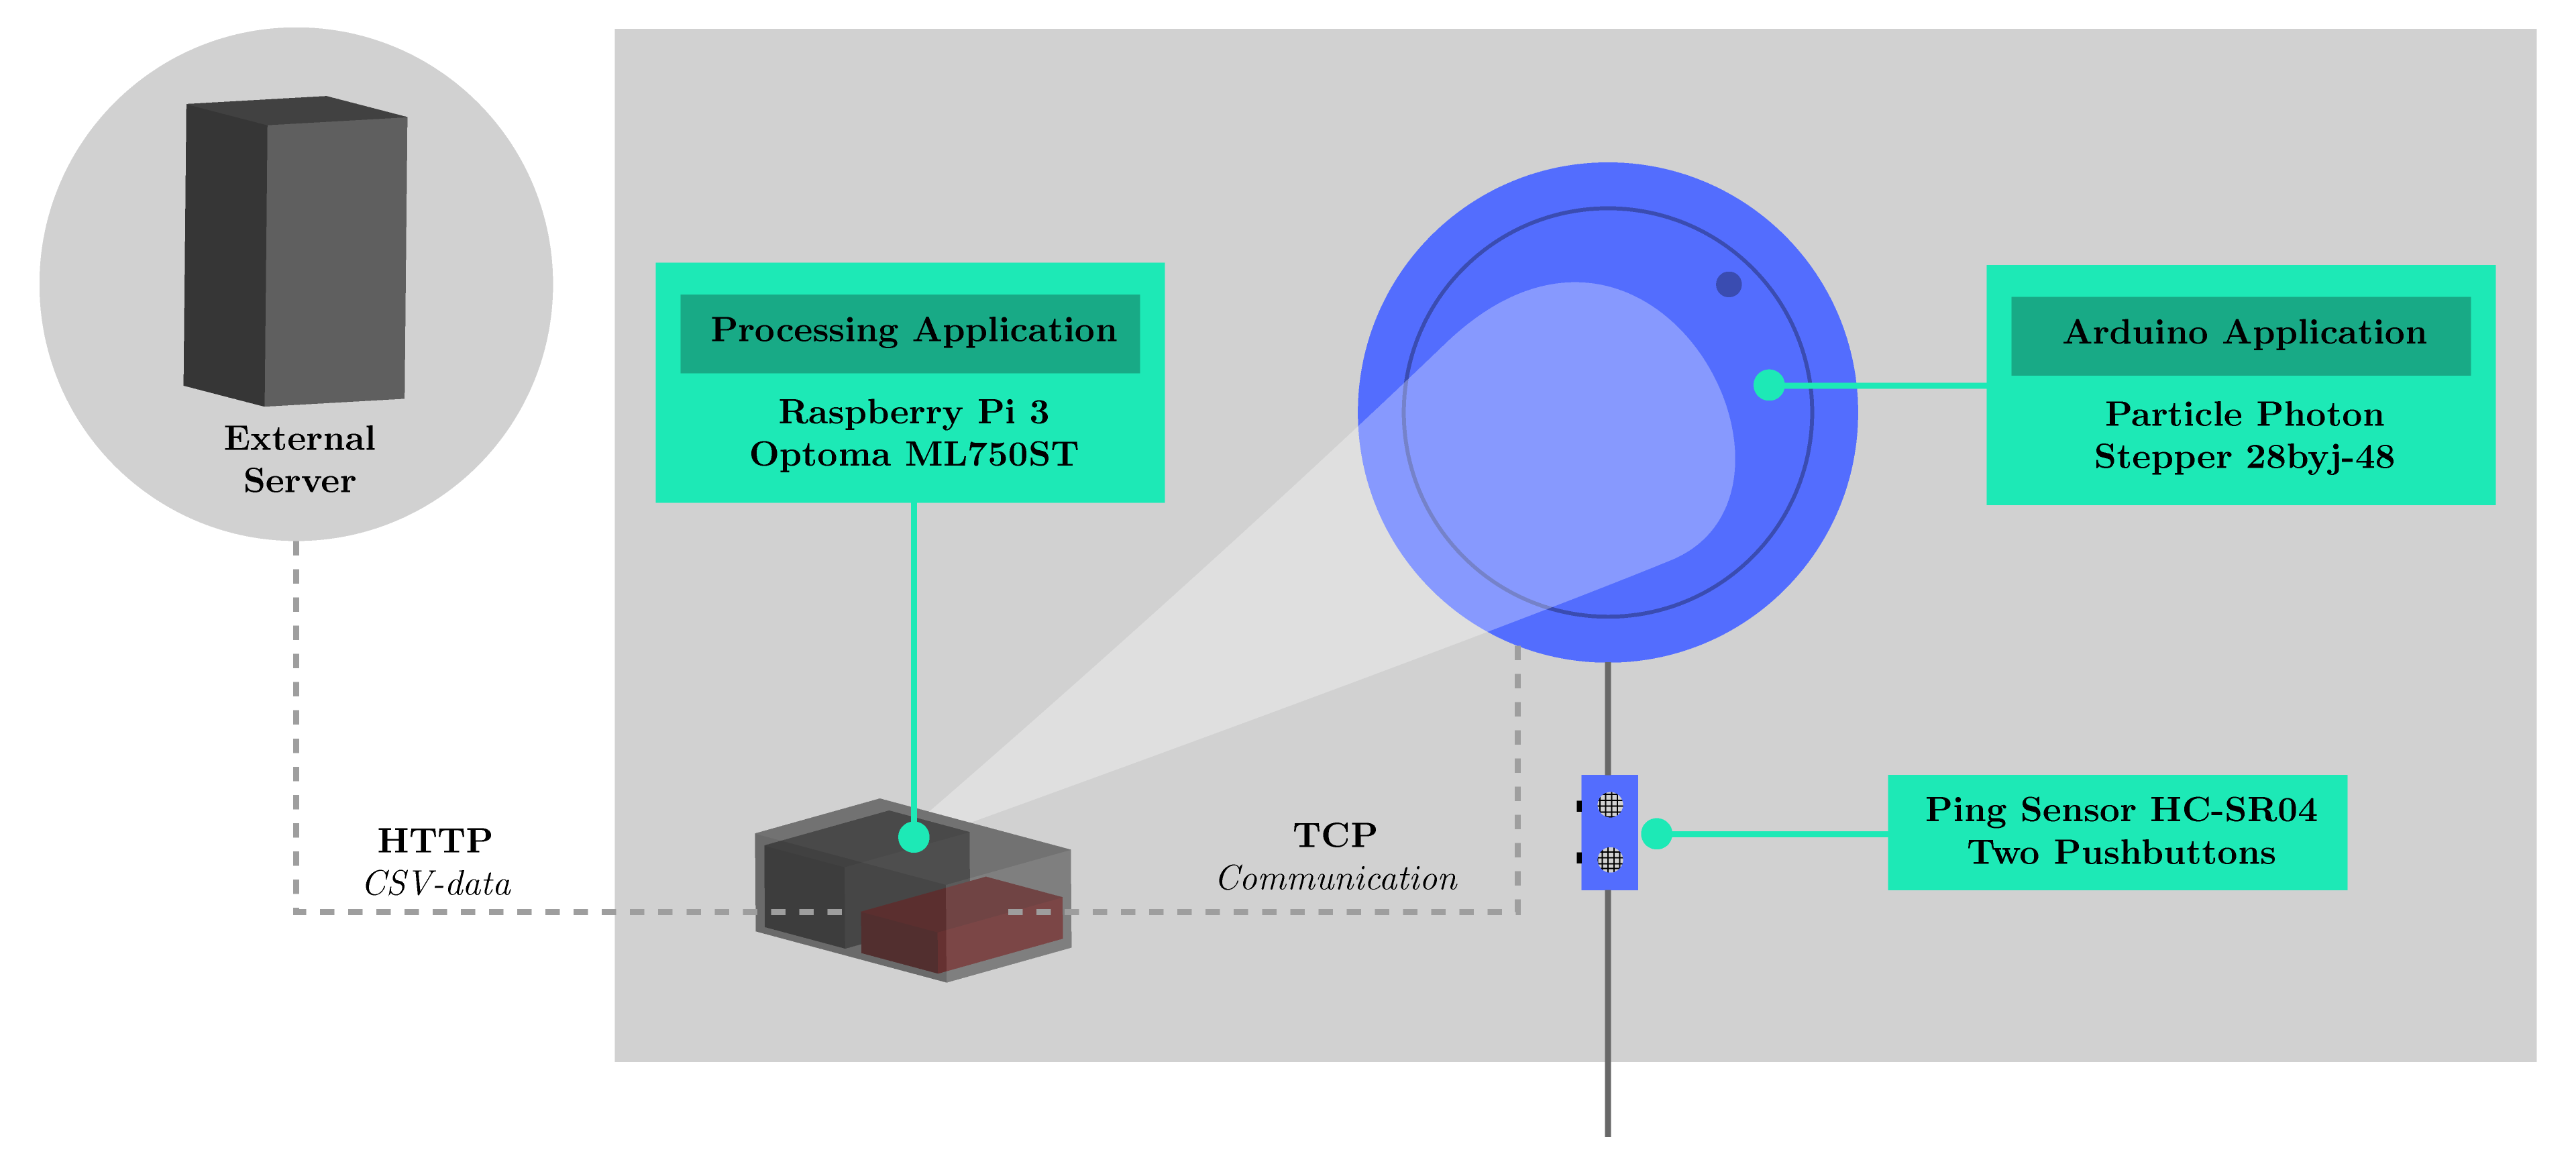
\includegraphics[width=\textwidth]{technical-diagram}
	\caption{Figure showing the technical implementation of the Financial Clock concept}
	\label{fig:technical-diagram}
\end{figure}

The Financial Clock prototype consists of two main parts; one part being the physical clock and the other a projector with a mounted Raspberry Pi (see figure figure~\ref{fig:technical-diagram}). The clock was laser cut from plywood in a circular shape with a diameter of 31 centimeters. Within this, the rotating dial was laser cut with a diameter of 25 centimeters. A small box containing a photon processor and a stepper motor was attached on the back of the clock with the stepper motor connected to the dial, allowing it to rotate smoothly with a granularity of 2048 steps per revolution. The clock is connected to a controller device, placed approximately 30 centimeters below it, through a cord. The controller device is equipped with two buttons on the side that rotates the dial clockwise and counterclockwise respectively as well as a HC-SR04 ping sensor used to make the display emerge when the user is in the proximity. The projector used to augment the clock is an Optoma ml750st with a WXGA resolution of 1280 x 800 pixels. This projector is small and portable with a short throw lens that enables it to be placed closely to the clock, which is preferred considering the prototype must be deployed in the homes of users where it is impossible to mount it in the ceiling, which we believe is the optimal placement, due to the inconvenience it would cause. On top of the projector is a Raspberry Pi 3 Model B that is connected to the projector via HDMI. The Raspberry Pi runs a Processing application which creates the graphic display that is projected onto the clock. The position of the display is manually calibrated upon setup of the prototype using the arrow keys, with the possibility to warp the display through corner pin keystoning, meaning that the projector can be positioned at an angle if needed.

Both the Raspberry Pi and the Photon are internet-connected devices that communicate using the TCP protocol. The Photon sends commands to the Raspberry Pi, telling it to turn the display on/off based on proximity sensing and interaction with the controller device. Furthermore it informs the Raspberry Pi to update the display according to the day the user inspects with the controller device. Finally, the Raspberry Pi continuously requests a server for the user’s latest financial data and updates the display when new data is available. In the current implementation we must manually retrieve the user’s data and upload it to this server as it is extremely difficult to automate this process due to the restrictions on sensitive financial data.
